%definira klasu dokumenta 
\documentclass[12pt]{report} 

%prostor izmedu naredbi \documentclass i \begin{document} se zove uvod. U njemu se nalaze naredbe koje se odnose na cijeli dokument

%osnovni LaTex ne može riješiti sve probleme, pa se koriste različiti paketi koji olakšavaju izradu željenog dokumenta
\usepackage[croatian]{babel} 
\usepackage{amssymb}
\usepackage{amsmath}
\usepackage{txfonts}
\usepackage{mathdots}
\usepackage{titlesec}
\usepackage{array}
\usepackage{lastpage}
\usepackage{etoolbox}
\usepackage{tabularray}
\usepackage{color, colortbl}
\usepackage{adjustbox}
\usepackage{geometry}
\usepackage[classicReIm]{kpfonts}
\usepackage{hyperref}
\usepackage{fancyhdr}

\usepackage{float}
\usepackage{setspace}
\restylefloat{table}


\patchcmd{\chapter}{\thispagestyle{plain}}{\thispagestyle{fancy}}{}{} %redefiniranje stila stranice u paketu fancyhdr

%oblik naslova poglavlja
\titleformat{\chapter}{\normalfont\huge\bfseries}{\thechapter.}{20pt}{\Huge}
\titlespacing{\chapter}{0pt}{0pt}{40pt}


\linespread{1.3} %razmak između redaka

\geometry{a4paper, left=1in, top=1in,}  %oblik stranice

\hypersetup{ colorlinks, citecolor=black, filecolor=black, linkcolor=black,	urlcolor=black }   %izgled poveznice


%prored smanjen između redaka u nabrajanjima i popisima
\newenvironment{packed_enum}{
	\begin{enumerate}
		\setlength{\itemsep}{0pt}
		\setlength{\parskip}{0pt}
		\setlength{\parsep}{0pt}
	}{\end{enumerate}}

\newenvironment{packed_item}{
	\begin{itemize}
		\setlength{\itemsep}{0pt}
		\setlength{\parskip}{0pt}
		\setlength{\parsep}{0pt}
	}{\end{itemize}}




%boja za privatni i udaljeni kljuc u tablicama
\definecolor{LightBlue}{rgb}{0.9,0.9,1}
\definecolor{LightGreen}{rgb}{0.9,1,0.9}

%Promjena teksta za dugačke tablice
\DefTblrTemplate{contfoot-text}{normal}{Nastavljeno na idućoj stranici}
\SetTblrTemplate{contfoot-text}{normal}
\DefTblrTemplate{conthead-text}{normal}{(Nastavljeno)}
\SetTblrTemplate{conthead-text}{normal}
\DefTblrTemplate{middlehead,lasthead}{normal}{Nastavljeno od prethodne stranice}
\SetTblrTemplate{middlehead,lasthead}{normal}

%podesavanje zaglavlja i podnožja

\pagestyle{fancy}
\lhead{Programsko inženjerstvo}
\rhead{CookBooked}
\lfoot{Culinary Chaos Crew}
\cfoot{stranica \thepage/\pageref{LastPage}}
\rfoot{\today}
\renewcommand{\headrulewidth}{0.2pt}
\renewcommand{\footrulewidth}{0.2pt}


\begin{document} 
	
	
	
	\begin{titlepage}
		\begin{center}
			\vspace*{\stretch{1.0}} %u kombinaciji s ostalim \vspace naredbama definira razmak između redaka teksta
			\LARGE Programsko inženjerstvo\\
			\large Ak. god. 2023./2024.\\
			
			\vspace*{\stretch{3.0}}
			
			\huge CookBooked\\
			\Large Dokumentacija, Rev. \textit{1}\\
			
			\vspace*{\stretch{12.0}}
			\normalsize
			Grupa: \textit{Culinary Chaos Crew}\\
			Voditelj: \textit{Dominik Dejanović}\\
			
			
			\vspace*{\stretch{1.0}}
			Datum predaje: \textit{17.11.2023.}\\
	
			\vspace*{\stretch{4.0}}
			
			Nastavnik: \textit{Nikolina Frid}\\
		
		\end{center}

	
	\end{titlepage}

	
	\tableofcontents


	\chapter{Dnevnik promjena dokumentacije}
		
		\textbf{\textit{Kontinuirano osvježavanje}}\\
				
		
		\begin{longtblr}[
				label=none
			]{
				width = \textwidth, 
				colspec={|X[2]|X[13]|X[3]|X[3]|}, 
				rowhead = 1
			}
			\hline
			\textbf{Rev.}	& \textbf{Opis promjene/dodatka} & \textbf{Autori} & \textbf{Datum}\\[3pt] \hline
			0.1 & Napravljen predložak.	& * & 22.08.2013. 		\\[3pt] \hline 
			0.2	& Dopisane upute za povijest dokumentacije.\newline Dodane reference. & * & 24.08.2013. 	\\[3pt] \hline 
			0.5 & Dodan \textit{Use Case} dijagram i jedan sekvencijski dijagram, funkcionalni i nefunkcionalni zahtjevi i dodatak A & * & 25.08.2013. \\[3pt] \hline 
			0.6 & Arhitektura i dizajn sustava, algoritmi i strukture podataka & * & 26.08.2013. \\[3pt] \hline 
			0.8 & Povijest rada i trenutni status implementacije,\newline Zaključci i plan daljnjeg rada & * & 28.08.2013. \\[3pt] \hline 
			0.9 & Opisi obrazaca uporabe & * & 07.09.2013. \\[3pt] \hline 
			0.10 & Preveden uvod & * & 08.09.2013. \\[3pt] \hline 
			0.11 & Sekvencijski dijagrami & * & 09.09.2013. \\[3pt] \hline 
			0.12.1 & Započeo dijagrame razreda & * & 10.09.2013. \\[3pt] \hline 
			0.12.2 & Nastavak dijagrama razreda & * & 11.09.2013. \\[3pt] \hline 
			\textbf{1.0} & Verzija samo s bitnim dijelovima za 1. ciklus & * & 11.09.2013. \\[3pt] \hline 
			1.1 & Uređivanje teksta -- funkcionalni i nefunkcionalni zahtjevi & * \newline * & 14.09.2013. \\[3pt] \hline 
			1.2 & Manje izmjene:Timer - Brojilo vremena & * & 15.09.2013. \\[3pt] \hline 
			1.3 & Popravljeni dijagrami obrazaca uporabe & * & 15.09.2013. \\[3pt] \hline 
			1.5 & Generalna revizija strukture dokumenta & * & 19.09.2013. \\[3pt] \hline 
			1.5.1 & Manja revizija (dijagram razmještaja) & * & 20.09.2013. \\[3pt] \hline 
			\textbf{2.0} & Konačni tekst predloška dokumentacije  & * & 28.09.2013. \\[3pt] \hline 
			&  &  & \\[3pt] \hline	
		\end{longtblr}
	
	
		\textit{Moraju postojati glavne revizije dokumenata 1.0 i 2.0 na kraju prvog i drugog ciklusa. Između tih revizija mogu postojati manje revizije već prema tome kako se dokument bude nadopunjavao. Očekuje se da nakon svake značajnije promjene (dodatka, izmjene, uklanjanja dijelova teksta i popratnih grafičkih sadržaja) dokumenta se to zabilježi kao revizija. Npr., revizije unutar prvog ciklusa će imati oznake 0.1, 0.2, …, 0.9, 0.10, 0.11.. sve do konačne revizije prvog ciklusa 1.0. U drugom ciklusu se nastavlja s revizijama 1.1, 1.2, itd.}
	\chapter{Opis projektnog zadatka}
		
		\textbf{\textit{Uvod}}\\
		
		\textit{Cilj ovog projekta je razviti CookBooked, platformu za zajednicu ljubitelja kuhanja i pečenja kolača, koja omogućava korisnicima razmjenu i otkrivanje recepata iz cijeloga svijeta. Autori recepata će dobiti priliku izgraditi svoju reputaciju, povećati svoju publiku i razmijeniti iskustva s drugima. To će stvoriti motivaciju za kontinuirano stvaranje visokokvalitetnih recepata i sadržaja. S druge strane, korisnici će dobiti priliku unaprijediti vlastite vještine i pričati s autorima recepata te dobiti inspiraciju za vlastite eksperimente u kuhinji. Programska potpora za aplikaciju implementirat će se u obliku web aplikacije.}
		
		\vspace{\baselineskip} % Add space equivalent to one line

		\textbf{\textit{Korisnički zahtjevi}}\\
		
		\textit{CookBooked je platforma koja zadovoljava raznolike potrebe korisnika. Navedeni su različiti tipovi korisnika i njihovi zahtjevi:}
		\begin{itemize}
			\item Item 1
			\item Item 2
			\item Item 3
		\end{itemize}
		
		\eject
		
	
	\chapter{Specifikacija programske potpore}
		
	\section{Funkcionalni zahtjevi}
			
			\textbf{\textit{dio 1. revizije}}\\
			
			\textit{Navesti \textbf{dionike} koji imaju \textbf{interes u ovom sustavu} ili  \textbf{su nositelji odgovornosti}. To su prije svega korisnici, ali i administratori sustava, naručitelji, razvojni tim.}\\
				
			\textit{Navesti \textbf{aktore} koji izravno \textbf{koriste} ili \textbf{komuniciraju sa sustavom}. Oni mogu imati inicijatorsku ulogu, tj. započinju određene procese u sustavu ili samo sudioničku ulogu, tj. obavljaju određeni posao. Za svakog aktora navesti funkcionalne zahtjeve koji se na njega odnose.}\\
			
			
			\noindent \textbf{Dionici:}
			
			\begin{packed_enum}
				
				\item Korisnik
				\item Administrator				
				\item Razvojni tim
				
			\end{packed_enum}
			
			\noindent \textbf{Aktori i njihovi funkcionalni zahtjevi:}
			
			
			\begin{packed_enum}
				\item  \underbar{Neregistrirani korisnik (inicijator) može: }
				\begin{packed_enum}
					\item vidjeti listu recepata svih korisnika
					\begin{packed_enum}
						\item filtrirati listu
						\item sortirati listu
					\end{packed_enum}
					\item pretraživati recepte po naslovu i korisniku
					\item napraviti novi račun
				\end{packed_enum}
			
				\item  \underbar{Registrirani korisnik (inicijator) može:}
				\begin{packed_enum}
					\item raditi nove recepte
					\item pregledati listu svojih recepata
					\item obrisati vlastiti recept
					\item promijeniti detalje računa:
					\begin{packed_enum}
						\item korisničko ime
						\item lozinku
					\end{packed_enum}
					\item deaktivirati račun
				\end{packed_enum}
			
				\item\underbar{Administrator (inicijator) može:}
				\begin{packed_enum}
					\item pregledati korisničke podatke
					\item pregledati recepte
					\item promijeniti korisničke podatke
					\item promijeniti podatke o receptu
					\item izbrisati korisnički račun
					\item izbrisati recept
				\end{packed_enum}
			
				\item\underbar{Baza podataka (sudionik):}
				\begin{packed_enum}
					\item pohranjuje podatke o:
					\begin{packed_enum}
						\item korisnicima
						\item receptima
					\end{packed_enum}
				\end{packed_enum}
			
				\item\underbar{API (sudionik):}
				\begin{packed_enum}
					\item omogućava dohvaćanje i strukturirano slanje podataka iz baze podataka
				\end{packed_enum}
			
				\item\underbar{Web stranica(sudionik):}
				\begin{packed_enum}
					\item omogućava korisnicima interakciju sa:
					\begin{packed_enum}
						\item drugim korisnicima
						\item listom recepata
					\end{packed_enum}
				\end{packed_enum}
			
			\end{packed_enum}
			
			\eject 
			
			
				
			\subsection{Obrasci uporabe}
				
				\textbf{\textit{dio 1. revizije}}
				
				\subsubsection{Opis obrazaca uporabe}
					\textit{Funkcionalne zahtjeve razraditi u obliku obrazaca uporabe. Svaki obrazac je potrebno razraditi prema donjem predlošku. Ukoliko u nekom koraku može doći do odstupanja, potrebno je to odstupanje opisati i po mogućnosti ponuditi rješenje kojim bi se tijek obrasca vratio na osnovni tijek.}\\



					\noindent \underbar{\textbf{UC1 - stvaranje korisničkog računa}}
					\begin{packed_item}
						\item \textbf{Glavni sudionik: korisnik}
						\item  \textbf{Cilj: stvaranje novog korisničkog računa}
						\item  \textbf{Sudionici: web stranica, API, baza podataka}
						\item  \textbf{Preduvjet: -}
						
						\item  \textbf{Opis osnovnog tijeka:}
						\item[] \begin{packed_enum}
							\item korisnik klikne na gumb za prijavu
							\item korisnik upiše  željeno korisničko ime i lozinku
							\item korisnik klikne na gumb "Registracija"
							\item šalje se zahtjev na API
							\item API zapisuje novog korisnika u bazu podataka
							\item ako je registracija uspješna web stranica se preusmjeri na homepage, ali sa korisnikom prijavljenim u sustav
						\end{packed_enum}
						
						\item  \textbf{Opis mogućih odstupanja:}
						\item[] \begin{packed_item}							
							\item[1.a] korisničko ime je zauzeto (već postoji)
							\begin{packed_enum}
								\item prikazuje se poruka "Korisničko ime zauzeto!"
							\end{packed_enum}
							\item[1.b] lozinka je slaba (sadrži manje od 6 znakova i/ili sadrži samo slova)
							\begin{packed_enum}
								\item prikazuje se poruka "Lozinka mora imati najmanje 6 znakova te barem jedan broj ili specijalan znak!"
							\end{packed_enum}
						\end{packed_item}
					\end{packed_item}


				
					\noindent \underbar{\textbf{UC2 - prijava u korisnički račun}}
					\begin{packed_item}
						\item \textbf{Glavni sudionik: korisnik}
						\item  \textbf{Cilj: prijava korisnika u vlastiti račun}
						\item  \textbf{Sudionici: web stranica, API, baza podataka}
						\item  \textbf{Preduvjet: -}
						
						\item  \textbf{Opis osnovnog tijeka:}
						\item[] \begin{packed_enum}
							\item korisnik klikne na gumb za prijavu
							\item korisnik unosi korisničko ime i lozinku
							\item korisnik klikne na gumb "Prijava"
							\item šalje se zahtjev sa korisničkim podacima na API
							\item API provjerava točnost podataka u bazi podataka
							\item u slučaju da je korisnik unijeo točne podatke, web stranica se preusmjeri na homepage sa korisnikom koji je sada prijavljen
						\end{packed_enum}
						
						\item  \textbf{Opis mogućih odstupanja:}
						\item[] \begin{packed_item}
							\item[2.a] korisničko ime ne postoji u bazi podataka
							\begin{packed_enum}
								\item prikazuje se poruka "Korisničko ime ne postoji!"
							\end{packed_enum}
							\item[2.b] pogrešna lozinka
							\begin{packed_enum}
								\item prikazuje se poruka "Kriva lozinka!"
							\end{packed_enum}
						\end{packed_item}
					\end{packed_item}


				
					\noindent \underbar{\textbf{UC3 - promjena korisničkih podataka}}
					\begin{packed_item}
						\item \textbf{Glavni sudionik: korisnik}
						\item  \textbf{Cilj: promjena korisničkog imena i/ili lozinke}
						\item  \textbf{Sudionici: web stanica, API, baza podataka}
						\item  \textbf{Preduvjet: korisnik je prijavljen u sustav}
						
						\item  \textbf{Opis osnovnog tijeka:}
						\item[] \begin{packed_enum}
							\item korisnik klikne na gumb "Postavke"
							\item[2.a] korisnik promijeni korisničko ime upisivanjem novog imena
							\item[2.b] korisnik promijeni lozinku upisivanjem nove lozinke 
							\item[3.] korisnik klikne na gumb "Pohrani promjene"
							\item[4.] šalje se zahtjev za promjenom podataka na API
							\item[5.] u bazu podataka se upisuju promjene
							\item[6.] korisnik se automatski odjavi za stranice
						\end{packed_enum}
						
						\item  \textbf{Opis mogućih odstupanja:}
						\item[] \begin{packed_item}
							\item[3.a] novo korisničko ime je zauzeto
							\begin{packed_enum}
								\item prikacuje se poruka "Korisničko ime zauzeto!"
							\end{packed_enum}
							\item[3.b] lozinka je slaba (sadrži manje od 6 znakova i/ili sadrži samo slova)
							\begin{packed_enum}
								\item prikazuje se poruka "Lozinka mora imati najmanje 6 znakova te barem jedan broj ili specijalan znak!"
							\end{packed_enum}
						\end{packed_item}
					\end{packed_item}
				
				
				
					\noindent \underbar{\textbf{UC4 - brisanje korisničkog računa}}
					\begin{packed_item}
						\item \textbf{Glavni sudionik: korisnik}
						\item  \textbf{Cilj: brisanje korisničkog računa i svih podataka vezanih uz račun}
						\item  \textbf{Sudionici: web stanica, API, baza podataka}
						\item  \textbf{Preduvjet: korisnik je prijavljen u sustav}
						
						\item  \textbf{Opis osnovnog tijeka:}
						\item[] \begin{packed_enum}
							\item korisnik klikne na gumb "Postavke"
							\item korisnik klikne na gumb "Obriši račun"
							\item pojavljuje se obavijest "Ovim postupkom će se obrisati svi Vaši receptii vaš račun, jesti li sigurni da želite nastaviti?"
							\item klikom na gumb "Da" se šalje zahtjev za brisanje računa API-u
							\item API briše račun iz baze podataka
							\item korisnik se preusmjerava na homepage, te više nije prijavljen u sustav
						\end{packed_enum}
						
						\item  \textbf{Opis mogućih odstupanja:}
						\item[] \begin{packed_item}							
							\item[4.a] korisnik kliknuo na gumb "Ne"
							\begin{packed_enum}
								\item obavijest se zatvara te korisnik ostaje u postavkama
							\end{packed_enum}
						\end{packed_item}
					\end{packed_item}



					\noindent \underbar{\textbf{UC5 - pregled liste recepata}}
					\begin{packed_item}
						\item \textbf{Glavni sudionik: korisnik}
						\item  \textbf{Cilj: prikazati recepte na web stranici}
						\item  \textbf{Sudionici: web stranica, baza podataka}
						\item  \textbf{Preduvjet: -}
						
						\item  \textbf{Opis osnovnog tijeka:}
						\item[] \begin{packed_enum}
							\item korisnik odabere filtere i način sortiranja recepata
							\item korisnik u polje za pretraživanje upiše tekst
							\item web stranica šalje zahtjev za dohvaćanje recepata API-u
							\item API dohvaća recepte iz baze podataka i šalje ih web stranici
							\item na web stranici se prikazuje lista recepata
						\end{packed_enum}
						
						\item  \textbf{Opis mogućih odstupanja:}
						\item[] \begin{packed_item}
							\item [5.a] nije upisan tekst po kojem se pretražuje
							\item[] \begin{packed_enum}
								\item prikazuju se svi recepti
							\end{packed_enum}
						\end{packed_item}
					\end{packed_item}


				
					\noindent \underbar{\textbf{UC6 - stvaranje novog recepta}}
					\begin{packed_item}
						\item \textbf{Glavni sudionik: korisnik}
						\item  \textbf{Cilj: kreiranje novog recepta}
						\item  \textbf{Sudionici: web stranica, API, baza podataka}
						\item  \textbf{Preduvjet: korisnik prijavljen u sustav}
						
						\item  \textbf{Opis osnovnog tijeka:}
						\item[] \begin{packed_enum}
							\item korisnik klikne na gumb "Novi recept"
							\item upišu se podaci o receptu kao postupak, slike, videi, kategorije itd.
							\item klikom na objavi recept se šalje zahtjev API-u
							\item API sprema recept u bazu podataka
							\item recept postaje vidljiv drugim korisnicima
						\end{packed_enum}
						
						\item  \textbf{Opis mogućih odstupanja:}
						\item[] \begin{packed_item}
							\item[6.a] recept nema naslov
							\begin{packed_enum}
								\item prikazuje se poruka "Potrebno je upisati ime recepta"
							\end{packed_enum}
							\item[6.b] nije upisana lista sastojaka
							\begin{packed_enum}
								\item prikazuje se poruka "Potrebno je upisati listu sastojaka"
							\end{packed_enum}
							\item[6.c] ne postoji ni jedan korak pripreme
							\begin{packed_enum}
								\item prikazuje se poruka "Potrebno je upisati barem jedan korak pripreme"
							\end{packed_enum}
							\item[6.d] nije uneseno vijeme kuhanja
							\begin{packed_enum}
								\item prikazuje se poruka "Potrebno je upisati vrijeme kuhanja"
							\end{packed_enum}
						\end{packed_item}
					\end{packed_item}



					\noindent \underbar{\textbf{UC7 - promjena podataka o receptu}}
					\begin{packed_item}
						\item \textbf{Glavni sudionik: korisnik}
						\item  \textbf{Cilj: promjena bilo kojeg podatka o receptu kojeg je korisnik napravio}
						\item  \textbf{Sudionici: web stranica, API, baza podataka}
						\item  \textbf{Preduvjet: korisnik je prijavljen u sustav te je on autor recepta kojeg želi promijeniti}
						
						\item  \textbf{Opis osnovnog tijeka:}
						\item[] \begin{packed_enum}
							\item korisnik klikne na svoj recept
							\item korisnik klikne na gumb za uređivanje recepta
							\item web stranica se preusmjerava na poveznicu za promjenu recepta
							\item[4.a] korisnik promijeni podatke o receptu i klikne gumb "Spremi promjene"
							\item[4.b] korisnik klikne na gumb "Izbriši recept"
							\item[5.] na API se šalje zahtjev sa novim podacima o receptu
							\item[6.] u bazu podataka se spremaju promjene
							\item[7.] web stranica se preusmjerava na poveznicu na kojoj se može pregledati recept ukoliko nije obrisan
						\end{packed_enum}
						
						\item  \textbf{Opis mogućih odstupanja:}
						\item[] \begin{packed_item}							
							\item[7.a] problem u novim podacima (referencirati se na odstupanja u UC6)
						\end{packed_item}
					\end{packed_item}



					\noindent \underbar{\textbf{UC8 - prijava na recepte korisnika}}
					\begin{packed_item}
						\item \textbf{Glavni sudionik: korisnika}
						\item  \textbf{Cilj: prijava korisnika na recepte autora kako bi primio obavijesti kada taj korisnik napravi novi recept}
						\item  \textbf{Sudionici: web stranica, API, baza podataka}
						\item  \textbf{Preduvjet: korisnik je prijavljen u sustav}
						
						\item  \textbf{Opis osnovnog tijeka:}
						\item[] \begin{packed_enum}
							\item prijavljeni korisnik otvara recept nekog autora
							\item klikom na gumb "???" se šalje zahtjev na API
							\item u bazu podataka se zapisuje da je korisnik prijavljen na recepte odabranog autora
							\item recepti autora se pokazuju u listi obavijesti
						\end{packed_enum}
						
						\item  \textbf{Opis mogućih odstupanja:}
						\item[] \begin{packed_item}							
							\item[8.a] korisnik je već prijavljen na recepte autora
							\begin{packed_enum}
								\item klikom na gumb za prijavu na recepte autora se korisnik odjavljuje sa recepata tog autora
							\end{packed_enum}
						\end{packed_item}
					\end{packed_item}
				
				
				
					\noindent \underbar{\textbf{UC9 - pregled obavijesti}}
					\begin{packed_item}
						\item \textbf{Glavni sudionik: korisnik}
						\item  \textbf{Cilj: pregled recepata autora koje korisnik prati}
						\item  \textbf{Sudionici: web stanica, API, baza podataka}
						\item  \textbf{Preduvjet: korisnik je prijavljen u sustav}
						
						\item  \textbf{Opis osnovnog tijeka:}
						\item[] \begin{packed_enum}
							\item korisnik klikne na gumb koji izgleda kao zvonce
							\item šalje se zahtjev na API
							\item iz baze podataka se čitaju obavijesti korisnika te se podaci vraćaju web stranici
							\item prikazuju se recepti svih autora koje korisnik prati
						\end{packed_enum}
						
						\item  \textbf{Opis mogućih odstupanja:}
						\item[] \begin{packed_item}							
						\end{packed_item}
					\end{packed_item}
				
				
				
					\noindent \underbar{\textbf{UC10 - spremanje/bookmarkanje recepta}}
					\begin{packed_item}
						\item \textbf{Glavni sudionik: korisnik}
						\item  \textbf{Cilj: spremanje recepata kako bi se kasnije mogli pregledati omiljeni recepti}
						\item  \textbf{Sudionici: web stanica, API, baza podataka}
						\item  \textbf{Preduvjet: korisnik prijavljen u sustav}
						
						\item  \textbf{Opis osnovnog tijeka:}
						\item[] \begin{packed_enum}
							\item[1.a] korisnik klikne na gumb za spremanje recepta iz liste recepata
							\item[1.b] korisnik klikne na gumb za spremanje recepata prilikom prikaza pojedinog recepta
							\item[2.] šalje se zahtjev na API
							\item[3.] u bazu podataka se upisuje recept kao omiljen od korisnika
						\end{packed_enum}
						
						\item  \textbf{Opis mogućih odstupanja:}
						\item[] \begin{packed_item}
							\item[10.a] recept je već spremljen kao omiljen
							\begin{packed_enum}
								\item recept se miče is liste omiljenih recepata
							\end{packed_enum}
						\end{packed_item}
					\end{packed_item}
				
				
				
					\noindent \underbar{\textbf{UC11 - pregled specifičnog recepta}}
					\begin{packed_item}
						\item \textbf{Glavni sudionik: korisnik}
						\item  \textbf{Cilj: prikaz svih podataka vezanih uz recept}
						\item  \textbf{Sudionici: web stranica, API, baza podataka}
						\item  \textbf{Preduvjet: -}
						
						\item  \textbf{Opis osnovnog tijeka:}
						\item[] \begin{packed_enum}
							\item korisnik kliknuo na recept
							\item šalje se zahtjev na API za dohvaćanje podataka o receptu
							\item iz baze podataka se čitaju podaci o receptu
							\item na web stranici se prikazuju dohvaćeni podaci
						\end{packed_enum}
						
						\item  \textbf{Opis mogućih odstupanja:}
						\item[] \begin{packed_item}							
						\end{packed_item}
					\end{packed_item}
					
					
					
					\noindent \underbar{\textbf{UC12 - komentiranje na recept}}
					\begin{packed_item}
						\item \textbf{Glavni sudionik: korisnik}
						\item  \textbf{Cilj: ostavlanje komentara na nekom receptu}
						\item  \textbf{Sudionici: web stranica, baza podataka}
						\item  \textbf{Preduvjet: korisnik je prijavljen u sustav te je otvorio stranicu recepta}
						
						\item  \textbf{Opis osnovnog tijeka:}
						\item[] \begin{packed_enum}
							\item scrollanjem do kraja recepta se dolazi do dijela sa komentarima
							\item upisuje se tekst u polje za komentar
							\item klikom na gumb "Objavi komentar" se šalje zahtjev na API
							\item u bazu podataka se upisuje komentar
							\item web stranica se osvježava
						\end{packed_enum}
						
						\item  \textbf{Opis mogućih odstupanja:}
						\item[] \begin{packed_item}
							\item[12.a] tekst komentara je prazno
							\begin{packed_enum}
								\item gumb za objavljivanje komentara je zasivljen te je nemoguće kliknuti na njega
							\end{packed_enum}
						\end{packed_item}
					\end{packed_item}
				
				
				
					\noindent \underbar{\textbf{UC}}
					\begin{packed_item}
						\item \textbf{Glavni sudionik: }
						\item  \textbf{Cilj:}
						\item  \textbf{Sudionici:}
						\item  \textbf{Preduvjet:}
						
						\item  \textbf{Opis osnovnog tijeka:}
						\item[] \begin{packed_enum}
						\end{packed_enum}
						
						\item  \textbf{Opis mogućih odstupanja:}
						\item[] \begin{packed_item}							
						\end{packed_item}
					\end{packed_item}
					
					
					
				\subsubsection{Dijagrami obrazaca uporabe}
					
					\textit{Prikazati odnos aktora i obrazaca uporabe odgovarajućim UML dijagramom. Nije nužno nacrtati sve na jednom dijagramu. Modelirati po razinama apstrakcije i skupovima srodnih funkcionalnosti.}
				\eject		
				
			\subsection{Sekvencijski dijagrami}
				
				\textbf{\textit{dio 1. revizije}}\\
				
				\textit{Nacrtati sekvencijske dijagrame koji modeliraju najvažnije dijelove sustava (max. 4 dijagrama). Ukoliko postoji nedoumica oko odabira, razjasniti s asistentom. Uz svaki dijagram napisati detaljni opis dijagrama.}
				\eject
	
		\section{Ostali zahtjevi}
		
			\textbf{\textit{dio 1. revizije}}\\
		 
			 \textit{Nefunkcionalni zahtjevi i zahtjevi domene primjene dopunjuju funkcionalne zahtjeve. Oni opisuju \textbf{kako se sustav treba ponašati} i koja \textbf{ograničenja} treba poštivati (performanse, korisničko iskustvo, pouzdanost, standardi kvalitete, sigurnost...). Primjeri takvih zahtjeva u Vašem projektu mogu biti: podržani jezici korisničkog sučelja, vrijeme odziva, najveći mogući podržani broj korisnika, podržane web/mobilne platforme, razina zaštite (protokoli komunikacije, kriptiranje...)... Svaki takav zahtjev potrebno je navesti u jednoj ili dvije rečenice.}
			 
			 
			 
	
	\chapter{Arhitektura i dizajn sustava}

\noindent Arhitekturu sustava dijelimo na tri različita dijela: \textbf{frontend}, \textbf{backend} i \textbf{bazu podataka}. Jedino koordinirana implementacija ovih podsustava zajedno dovodi do finalnog proizvoda u obliku web platforme koju ostvarujemo. 
\newline \newline
\noindent \textbf{\textit{Frontend}} predstavlja sučelje između korisnika i same platforme. Konkretno, on pruža korisniku pregled sadržaja web stranice i omogućava mu komunikaciju s aplikacijom putem \textit{HTTP} (\textit{HyperText Transfer Protocol}) zahtjeva.
\newline\newline\noindent \textbf{\textit{Backend}} je taj koji te zahtjeve obrađuje i upravlja podatcima u bazi podataka. Neke od funkcionalnosti koje omogućuje backend su primjerice registracija novog korisnika ili brisanje korisnika od strane sistemskog administratora. 
\newline\newline\noindent \textbf{\textit{Baza podataka}} spremište je entiteta koji su prikazani u obliku tablica s atributima. Iz nje se često čitaju podatci i po potrebi ažuriraju. Kritičan je dio arhitekture sustava. 
 \textbf{\newline\newline\noindent Controller - Service - Repository} troslojna arhitektura temelj je backend implementacije aplikacije. \textit{Controller} sloj povezuje frontend i backend, pozivajući \textit{Service} sloj da obradi zahtjeve korisnika. Ako je za obradu tih zahtjeva potreban pristup bazi podataka, Service sloj poziva funkcije \textit{Repository} sloja koji to omogućuje. 
 \newline\newline\noindent Frontend je implementiran uz pomoć \textit{JavaScripta} (radnog okvira \textit{React.js}), \textit{HTML-a} i \textit{CSS-}a. Za backend je korišten programski jezik \textit{Java} (radni okvir \textit{Spring Boot}), a odabrana je razvojna okolina \textit{Intellij IDEA}. Ispitivanje backend funkcionalnosti omogućeno je korištenjem \textit{Postman} platforme. Baza podataka izgrađena je korištenjem \textit{PostgreSQL} sustava za upravljanje bazom podataka. Aplikacija je stavljena u pogon na \textit{Render} servisu. 

		\section{Baza podataka}
			
		Za našu platformu koristit ćemo relacijsku bazu podataka. Objekt takve baze je relacija, odnosno tablica koja je definirana svojim imenom i skupom atributa. Atributi unutar jednog entiteta mogu poprimiti funkciju primarnog ili stranog ključa.
Baza podataka u našem se slučaju sastoji se od 2 entiteta - \textbf{profile} i \textbf{recipe}.
		
			\subsection{Opis tablica}

\noindent \textbf{\textit{profile}}\\
\begin{samepage}
Ovaj entitet sadrži osnovne informacije o korisničkom profilu i  sastoji se od sljedećih atributa: \textit{userID} (autogenerirani identifikator korisnika), \textit{email }(e-mail adresa), \textit{username} (korisničko ime), \textit{password} (lozinka), \textit{name} (ime), \textit{surname} (prezime) i \textit{age} (dob). Atribut\textit{ userID} primarni je ključ entiteta \textbf{profile}. 
\end{samepage}

    				\begin{longtblr}[
					label=none,
					entry=none
					]{
						width = \textwidth,
						colspec={|X[6,l]|X[6, l]|X[20, l]|}, 
						rowhead = 1,
					} %definicija širine tablice, širine stupaca, poravnanje i broja redaka naslova tablice
     
					\hline \SetCell[c=3]{c}{\textbf{profile}}	 \\ \hline[3pt]
					\SetCell{LightGreen}userID & VARCHAR	&  	jedinstveni identifikator korisnika	\\ \hline
					\SetCell{}email & VARCHAR	&  	jedinstvena e-mail adresa korisnika 	\\ \hline
     				\SetCell{}username & VARCHAR	&  	jedinstveno korisničko ime	\\ \hline
					\SetCell{} password & VARCHAR	&  lozinka korisnika 	\\ \hline
          			\SetCell{} name & VARCHAR	&  ime korisnika (opcionalno)	\\ \hline
               		\SetCell{} surname & VARCHAR	&  	prezime korisnika (opcionalno)	\\ \hline
                    \SetCell{} age & INT	&  	dob korisnika (opcionalno)	\\ \hline
                    
				\end{longtblr}

    
\noindent \textbf{\textit{recipe}}\\
\begin{samepage}
Ovaj entitet opisuje recept postavljen na platformu od strane registriranog korisnika. Primarni je ključ entiteta \textit{recipeID} (autogenerirani identifikator recepta), a strani ključ \textit{userID} koji povezuje entitete \textbf{recipe} i \textbf{profile}.
\end{samepage}
\eject

\begin{samepage}
\noindent Ostali atributi su: \textit{likes} (broj oznaka "sviđa mi se" na receptu od strane registriranih korisnika), koji je inicijalno postavljen na 0, \textit{ingredients} (sastojci jela koje recept opisuje), \textit{name} (ime recepta), \textit{instructions} (niz uputa pripreme jela opisanog receptom), \textit{origin} (mjesto podrijetla jela), \textit{category} (kategorija jela), \textit{specialTags} (dodatne oznake), \textit{imageURL} (URL slike koju korisnik prilaže uz postavljeni recept), \textit{videoURL} (URL videa koji korisnik prilaže uz postavljeni recept) te \textit{preparationTime} (vrijeme potrebno za spremanje receptnog jela).
\end{samepage}
    
    				\begin{longtblr}[
					label=none,
					entry=none
					]{
						width = \textwidth,
						colspec={|X[8, l]|X[6, l]|X[20, l]|}, 
						rowhead = 1,
					} %definicija širine tablice, širine stupaca, poravnanje i broja redaka naslova tablice
					\hline \SetCell[c=3]{c}{\textbf{recipe}}	 \\ \hline[3pt]
					\SetCell{LightGreen}recipeID & VARCHAR	&  	jedinstveni identifikator recepta 	\\ \hline
               		\SetCell{} likes & INT	&  	broj oznaka "sviđa mi se" recepta 	\\ \hline
                    \SetCell{} ingredients & VARCHAR	&  	popis sastojaka receptnog jela 	\\ \hline
                    \SetCell{} name & VARCHAR	&  	ime recepta 	\\ \hline
                    \SetCell{} instructions & VARCHAR	&  	niz uputa za pripremu jela prema receptu 	\\ \hline
                    \SetCell{} origin & VARCHAR	&  	mjesto podrijetla receptnog jela (opcionalno)	\\ \hline
                    \SetCell{} category & VARCHAR	&  	vrsta (kategorija) receptnog jela	\\ \hline
                    \SetCell{} specialTags & VARCHAR	&  	specijalne dodatne oznake receptnog jela (opcionalno)	\\ \hline
                    \SetCell{} imageURL & VARCHAR	&  	URL slike priložene uz recept 	\\ \hline
					\SetCell{} videoURL & VARCHAR	&  	URL videa priloženog uz recept (opcionalno)	\\ \hline
    				\SetCell{} preparationTime & INT	&  	vrijeme kuhanja jela u minutama	\\ \hline
					\SetCell{LightBlue}userID & VARCHAR	&  	jedinstveni identifikator korisnika 	\\ \hline
				\end{longtblr}
				
				
			
			\subsection{Dijagram baze podataka}
			
			\begin{figure}[H]
			    \centering
			    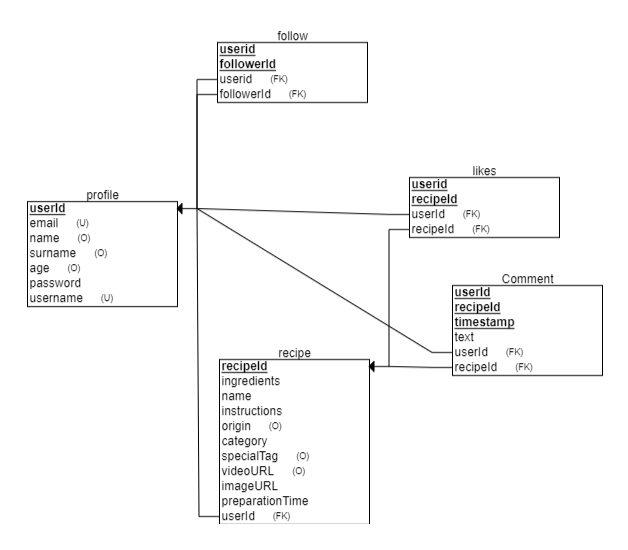
\includegraphics[width=1\linewidth]{slike/DBdiagram.png}
			    \caption{Dijagram baze podataka}
			    \label{fig:enter-label}
			\end{figure}
			
			\eject
			
			
		\section{Dijagram razreda}
			

\begin{figure}[H]
			    \centering
			    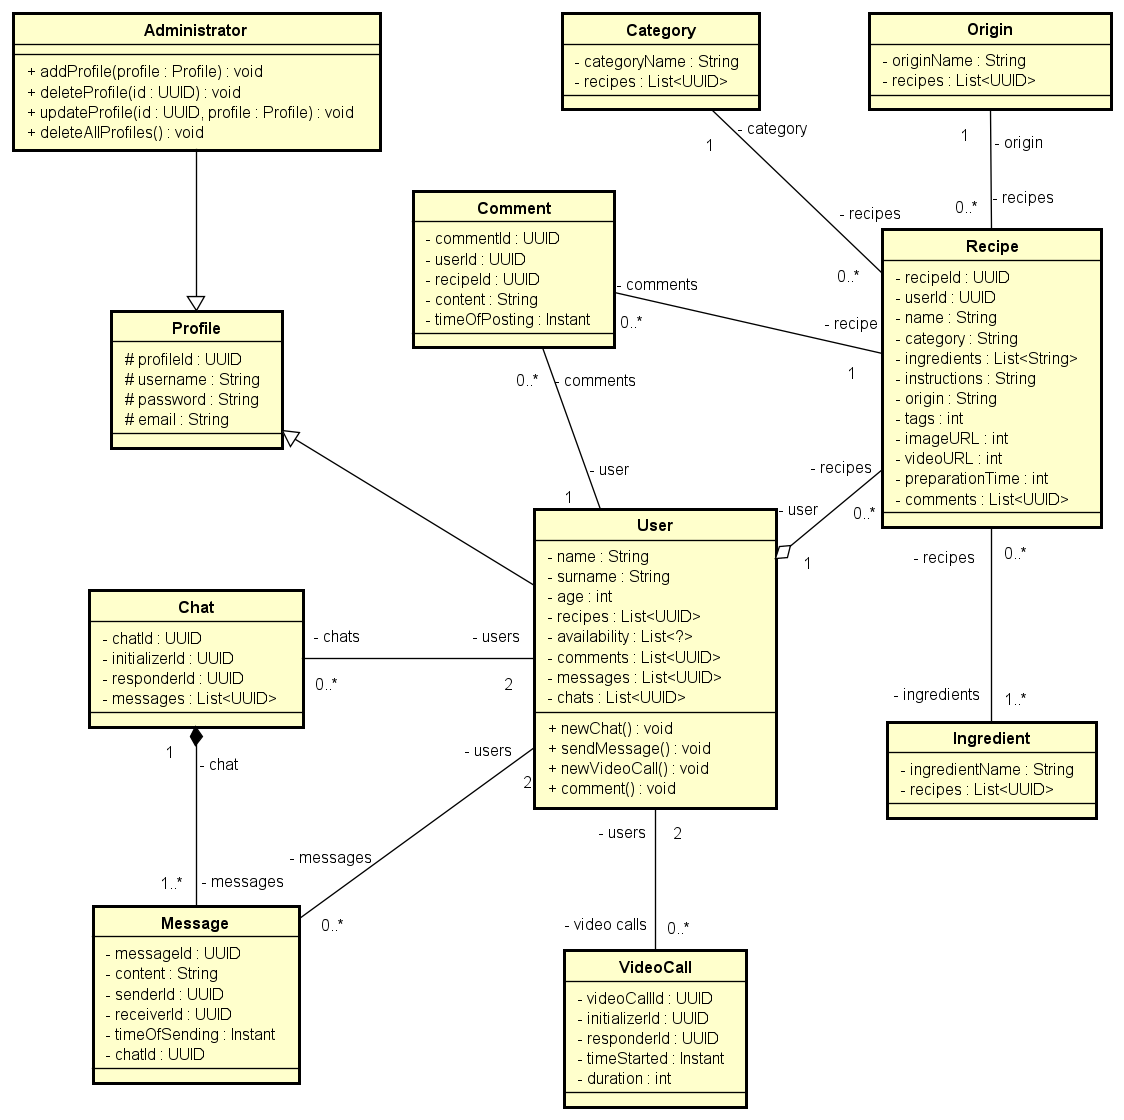
\includegraphics[width=1\linewidth]{slike//dijagrami/genericFunctionalityClassDiagram.png}
			    \caption{Dijagram razreda - generička funkcionalnost}
			    \label{fig:enter-label}
			\end{figure}
	\eject		
 \begin{figure}[H]
			    \centering
			    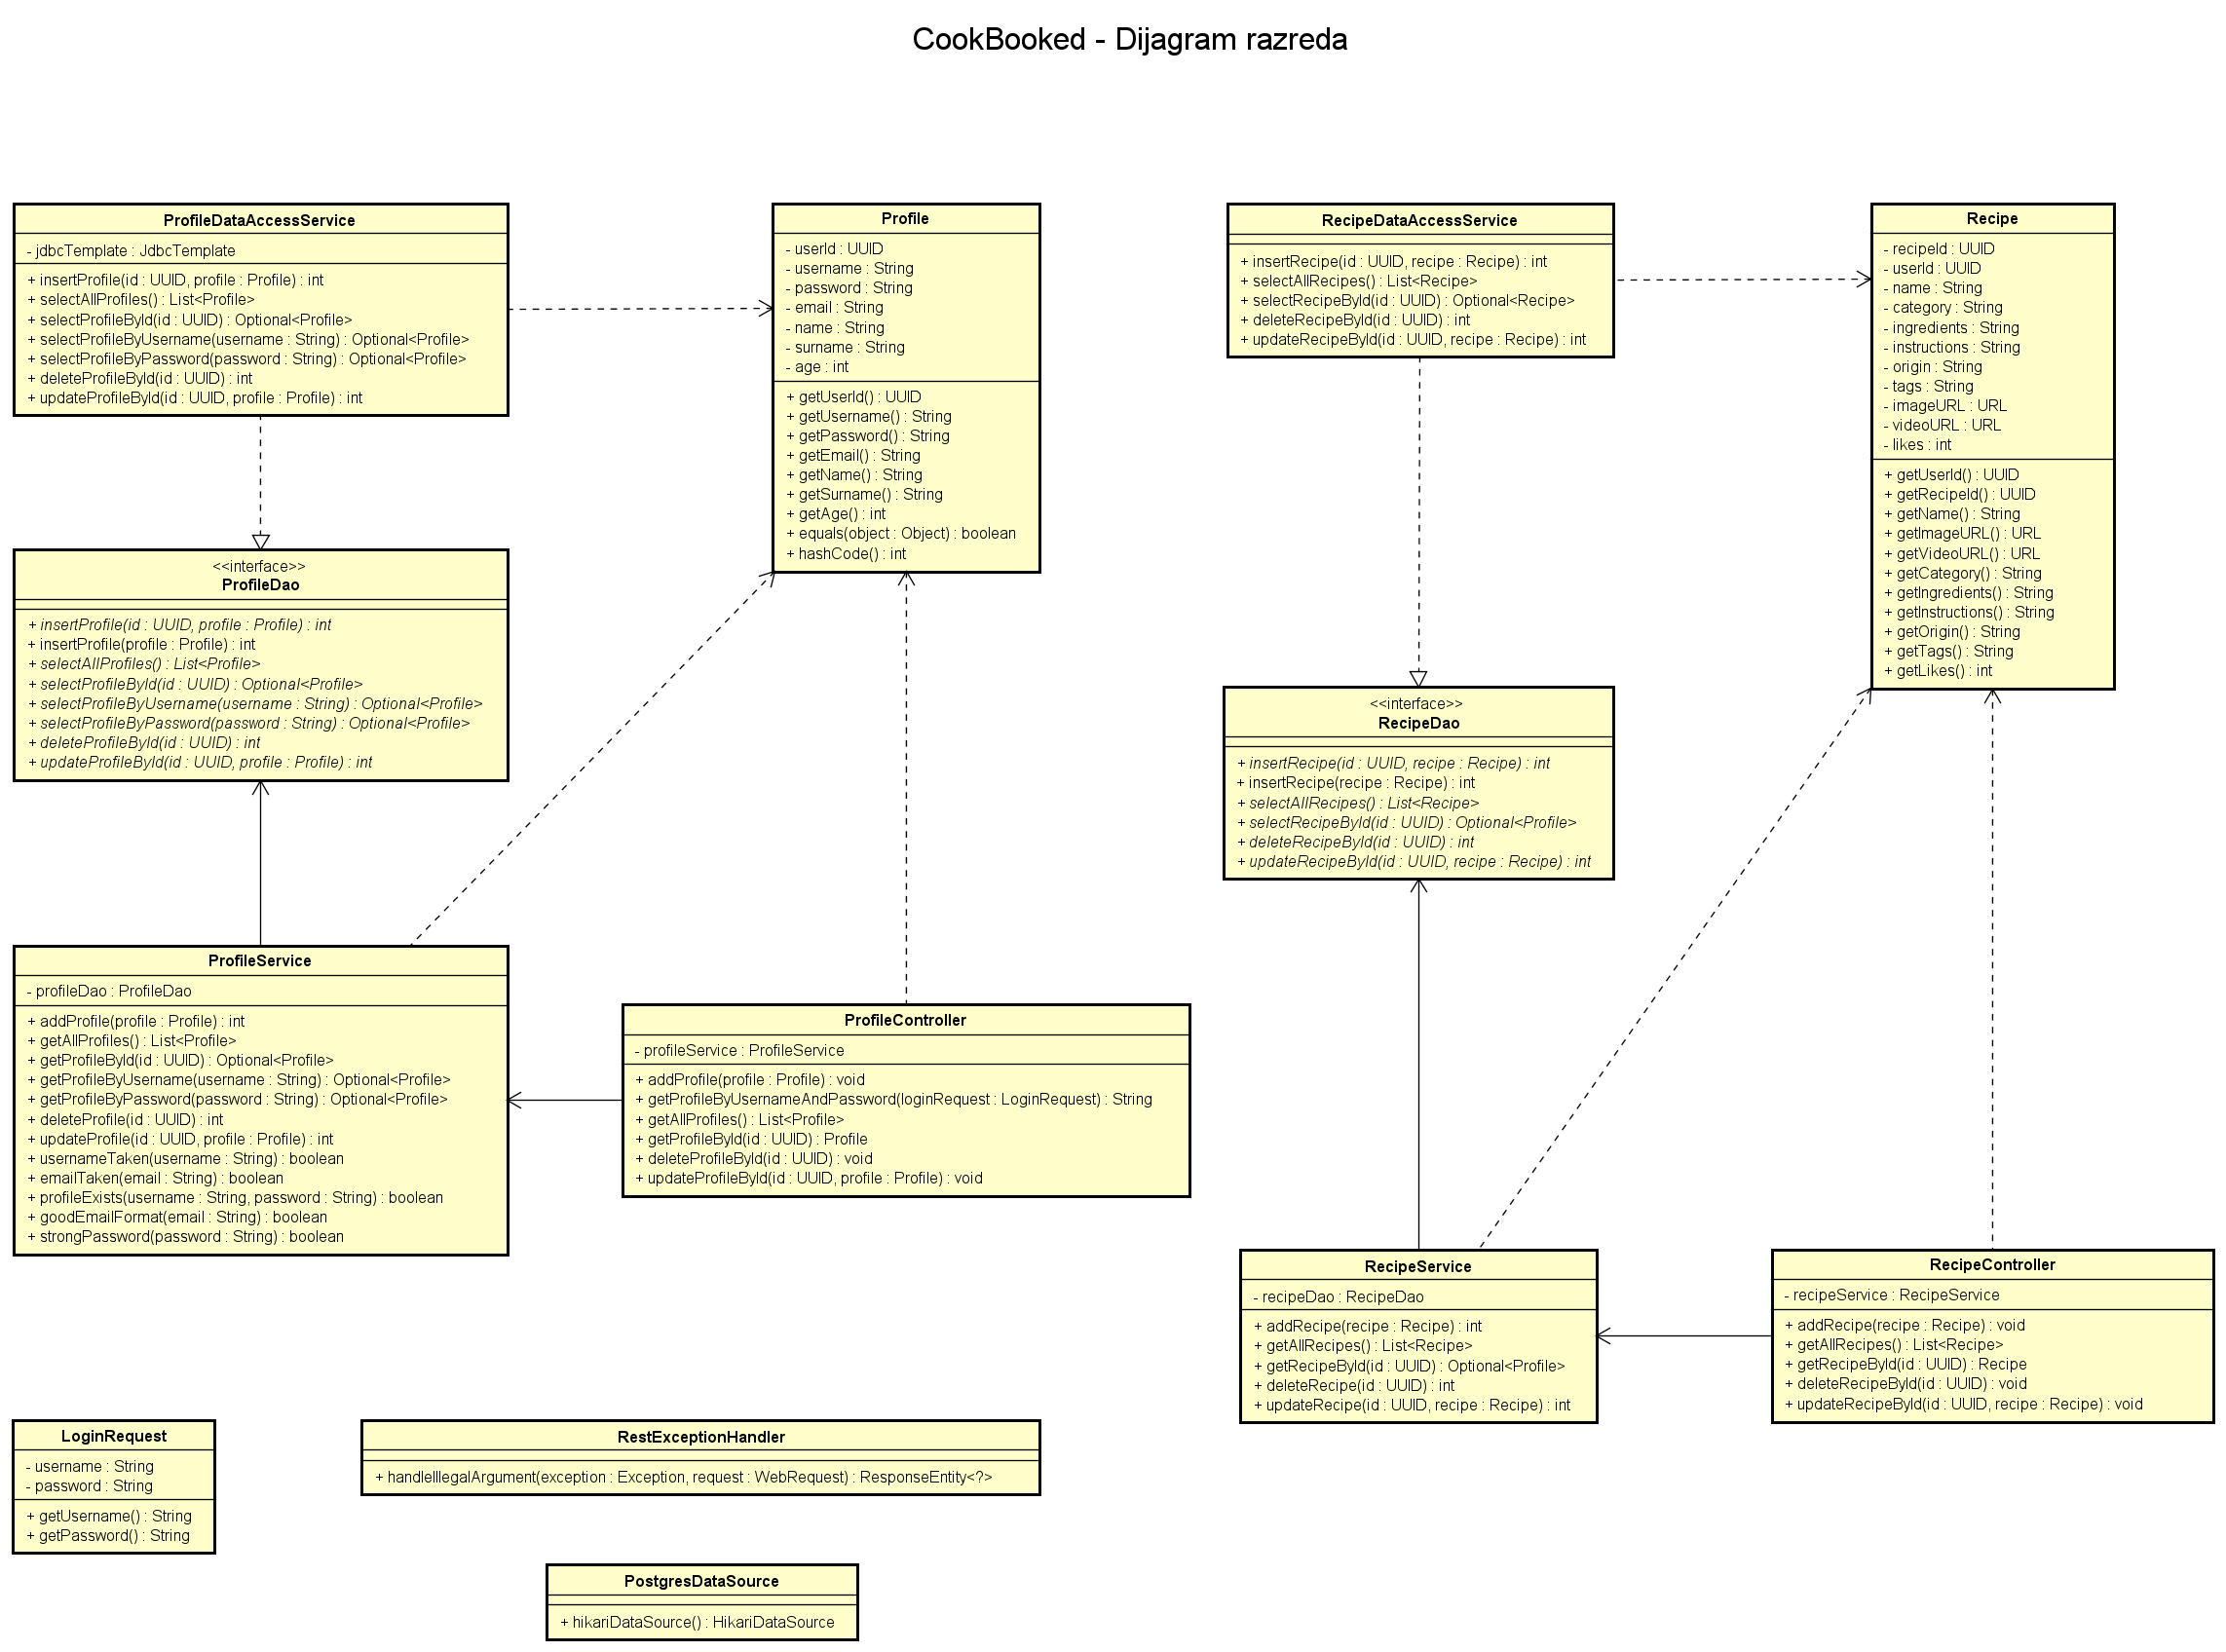
\includegraphics[width=1\linewidth]{slike/dijagrami/Dijagram razreda.png}
			    \caption{Dijagram razreda - trenutna implementacija u trenutku 1. revizije}
			    \label{fig:enter-label}
			\end{figure}
   \eject
   \textbf{\textit{dio 2. revizije}}\\			
			
			\textit{Prilikom druge predaje projekta dijagram razreda i opisi moraju odgovarati stvarnom stanju implementacije}
			
			
			
			\eject
		
		\section{Dijagram stanja}

		\noindent Dijagram stanja prikazuje stanja prijavljenog i neprijavljenog korisnika. Korisnik inicijalno nije prijavljen. Neprijavljeni korisnik iz home pagea ima opciju stisnuti gumb za pretraživanje novih recepata ili pregledavati recepte (ako ih ima) temeljem kategorija (npr. predjela, deserti), vrsta kuhinje (talijanska, kineska) ili specifičnih sastojaka uz pomoć tražilice. Neprijavljeni korisnik također može potražiti autora recepta temeljem korisničkog imena putem tražilice. Za pristup svim ostalim mogućnostima platforme, korisnik se mora registrirati ili prijaviti. Prijavljeni korisnik može sve što i neprijavljeni korisnik, a može koristiti i još neke stvari. Može stisnuti za gumb za dodavanje vlastitog recepta ili na gumb za pregled svih recepata koje je spremio. Također je moguće i pregledati te uređivati vlastiti profil na stranici profila. Još jedna pogodnost koju prijavljeni korisnici imaju je ta da mogu komunicirati s autorima putem chata ili videopoziva. Naravno, korisnik u bilo kojem trenutku može stisnuti na gumb s logoim stranice kako bi se vratio na Home page. 

		\eject
			
			\begin{figure}[H]
				\centering
				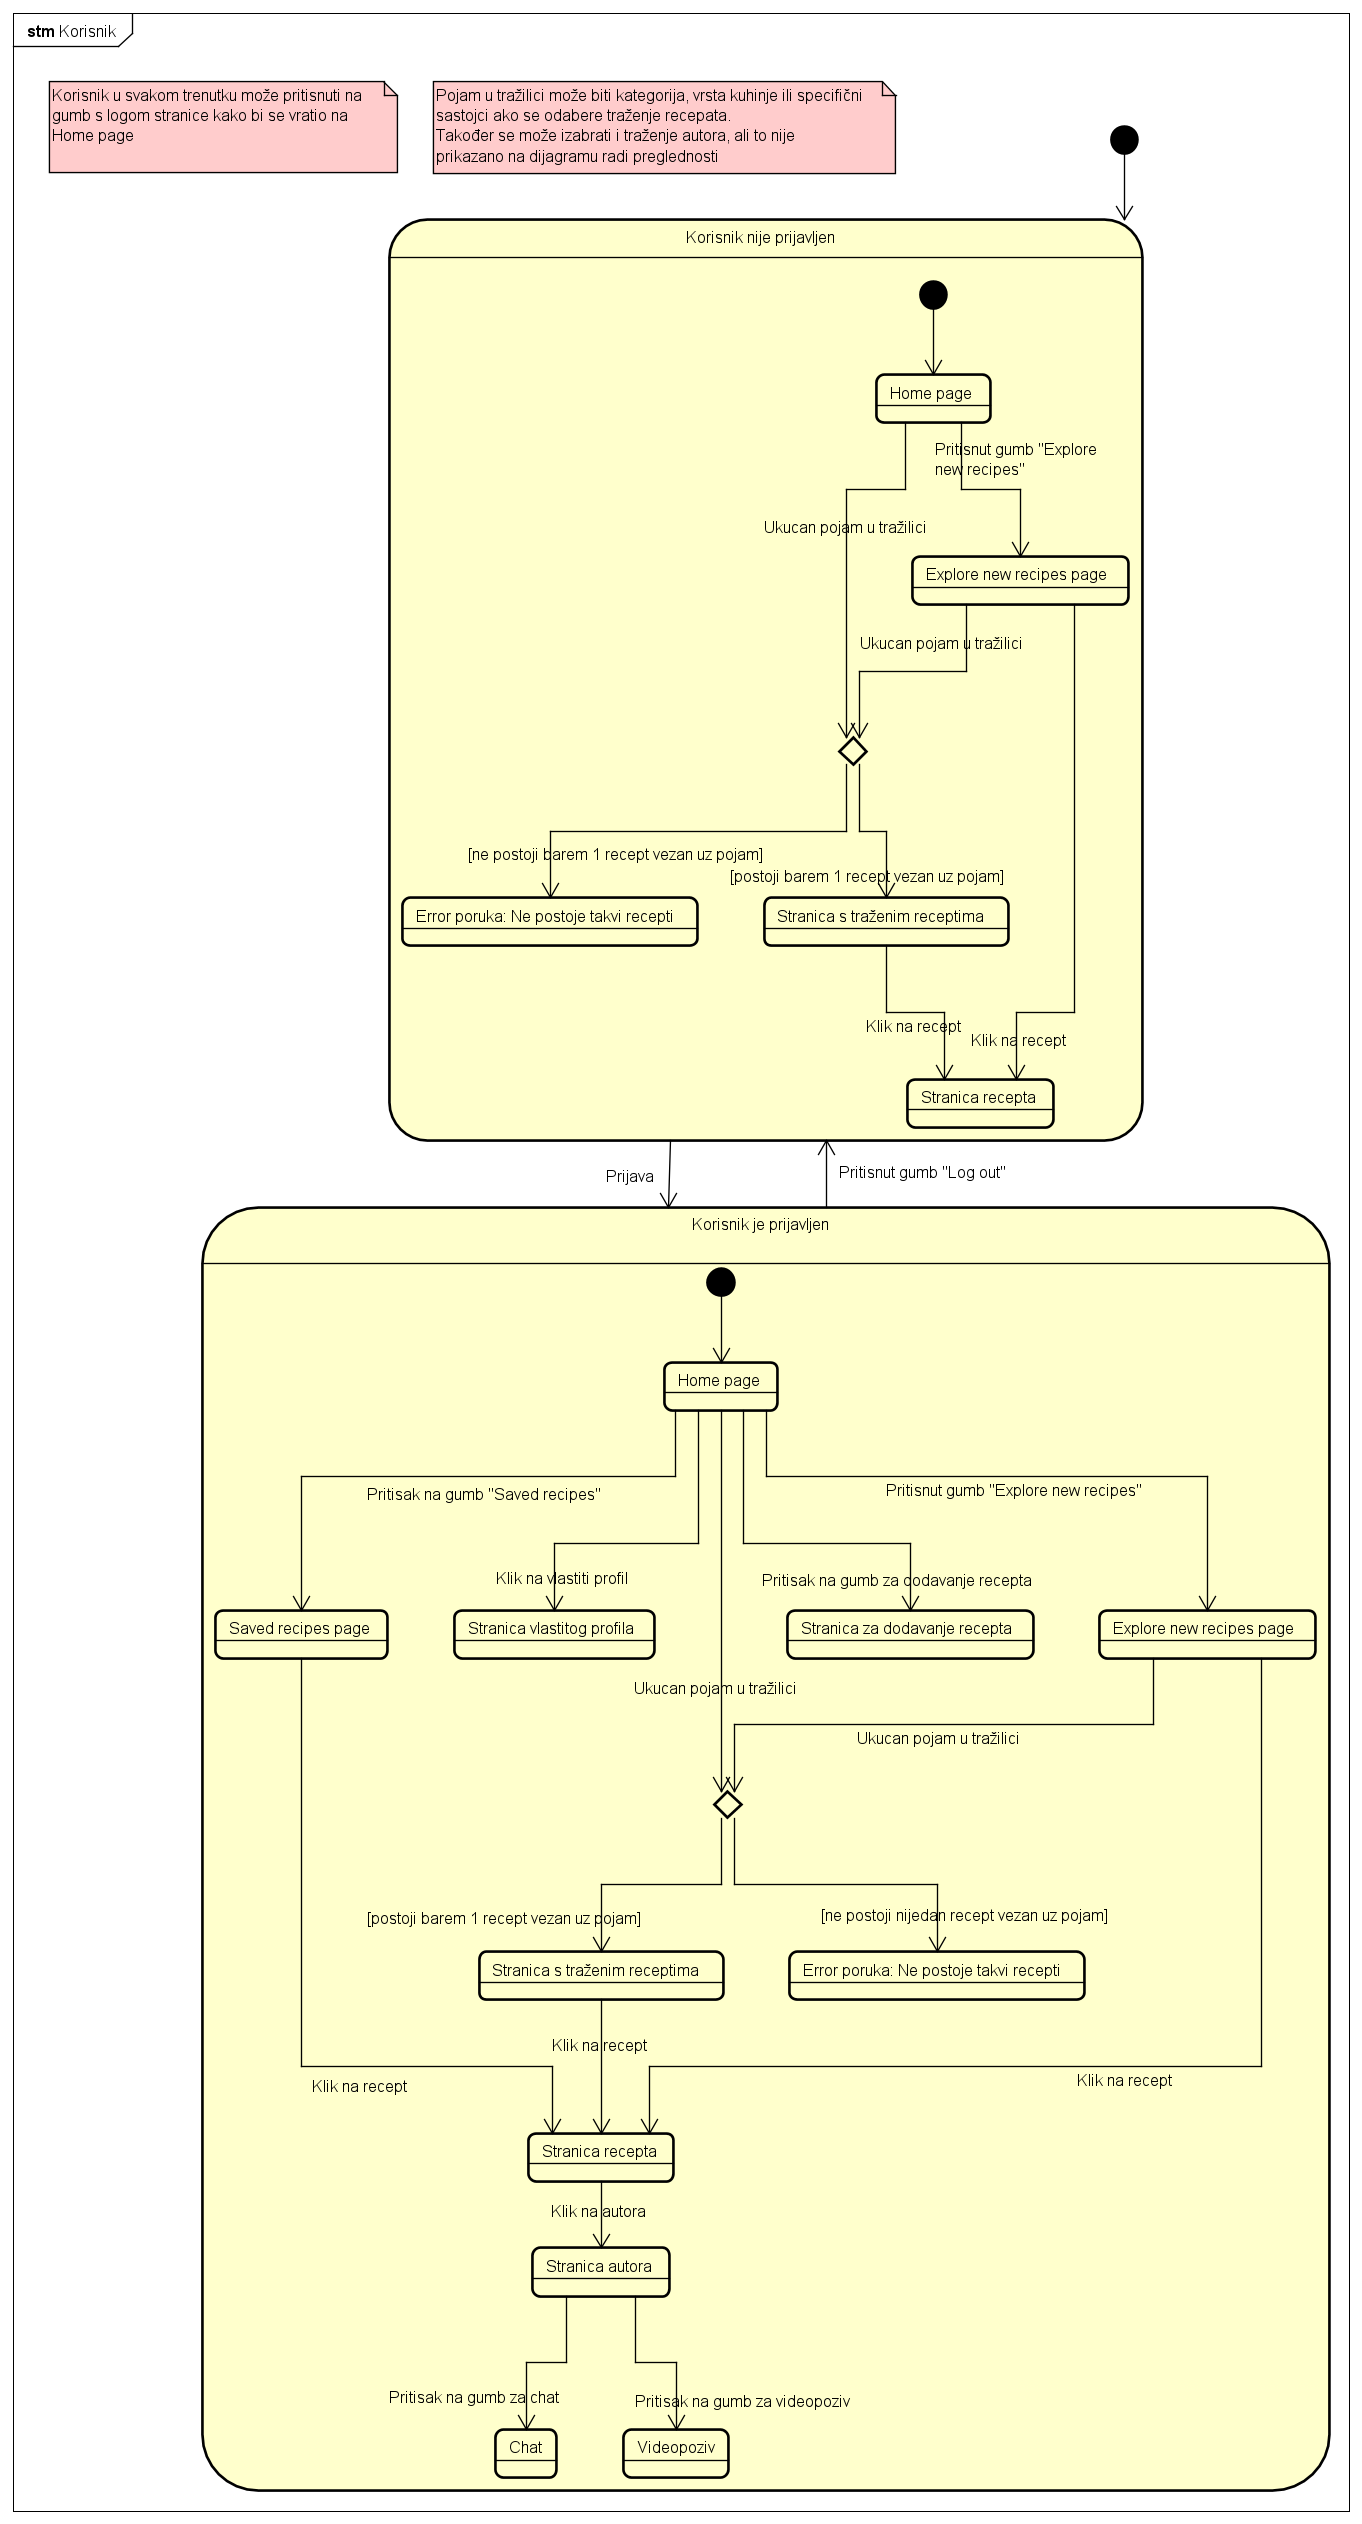
\includegraphics[height=0.95\textheight]{slike/dijagrami/Korisnik_dijagram_stanja.png}
				\caption{Dijagram stanja za korisnika}
				\label{fig:enter-label}
			\end{figure}
			
			
			\eject 
		
		\section{Dijagram aktivnosti}
			
		\noindent Dijagram aktivnosti prikazuje aktivnosti pregledavanja nespremljenih recepata i autora. Korisnik može naći nove recepte uz pomoć gumba "Explore new recipes" ili uz pomoć pretraživanja pojmova u tražilici. Kada korisnik odabere jednu od ovih dviju opcija, web aplikacija šalje upit za dohvat tih recepata bazi podataka koja daje odgovor o tome postoje li podaci i ako da, onda ih vraća. Nakon toga aplikacija prikazuje recepte na koje korisnik može kliknuti kako bi ih pohranio ili kako bi ih detaljnije pregledao. Naravno, u oba slučaja aplikacija mora slati upit bazi podataka kako bi dohvatila / pohranila podatke. Osim toga, korisnik u tražilici može pretraživati i autore pa tada baza dohvaća podatke iz tablice profiles. Nakon dohvaćanja autora, aplikacija prikazuje njegovu stranicu koja sadrži njegove podatke i recepte koje korisnik opet može pregledati i pohraniti.   

		\eject
			
			\begin{figure}[H]
				\centering
				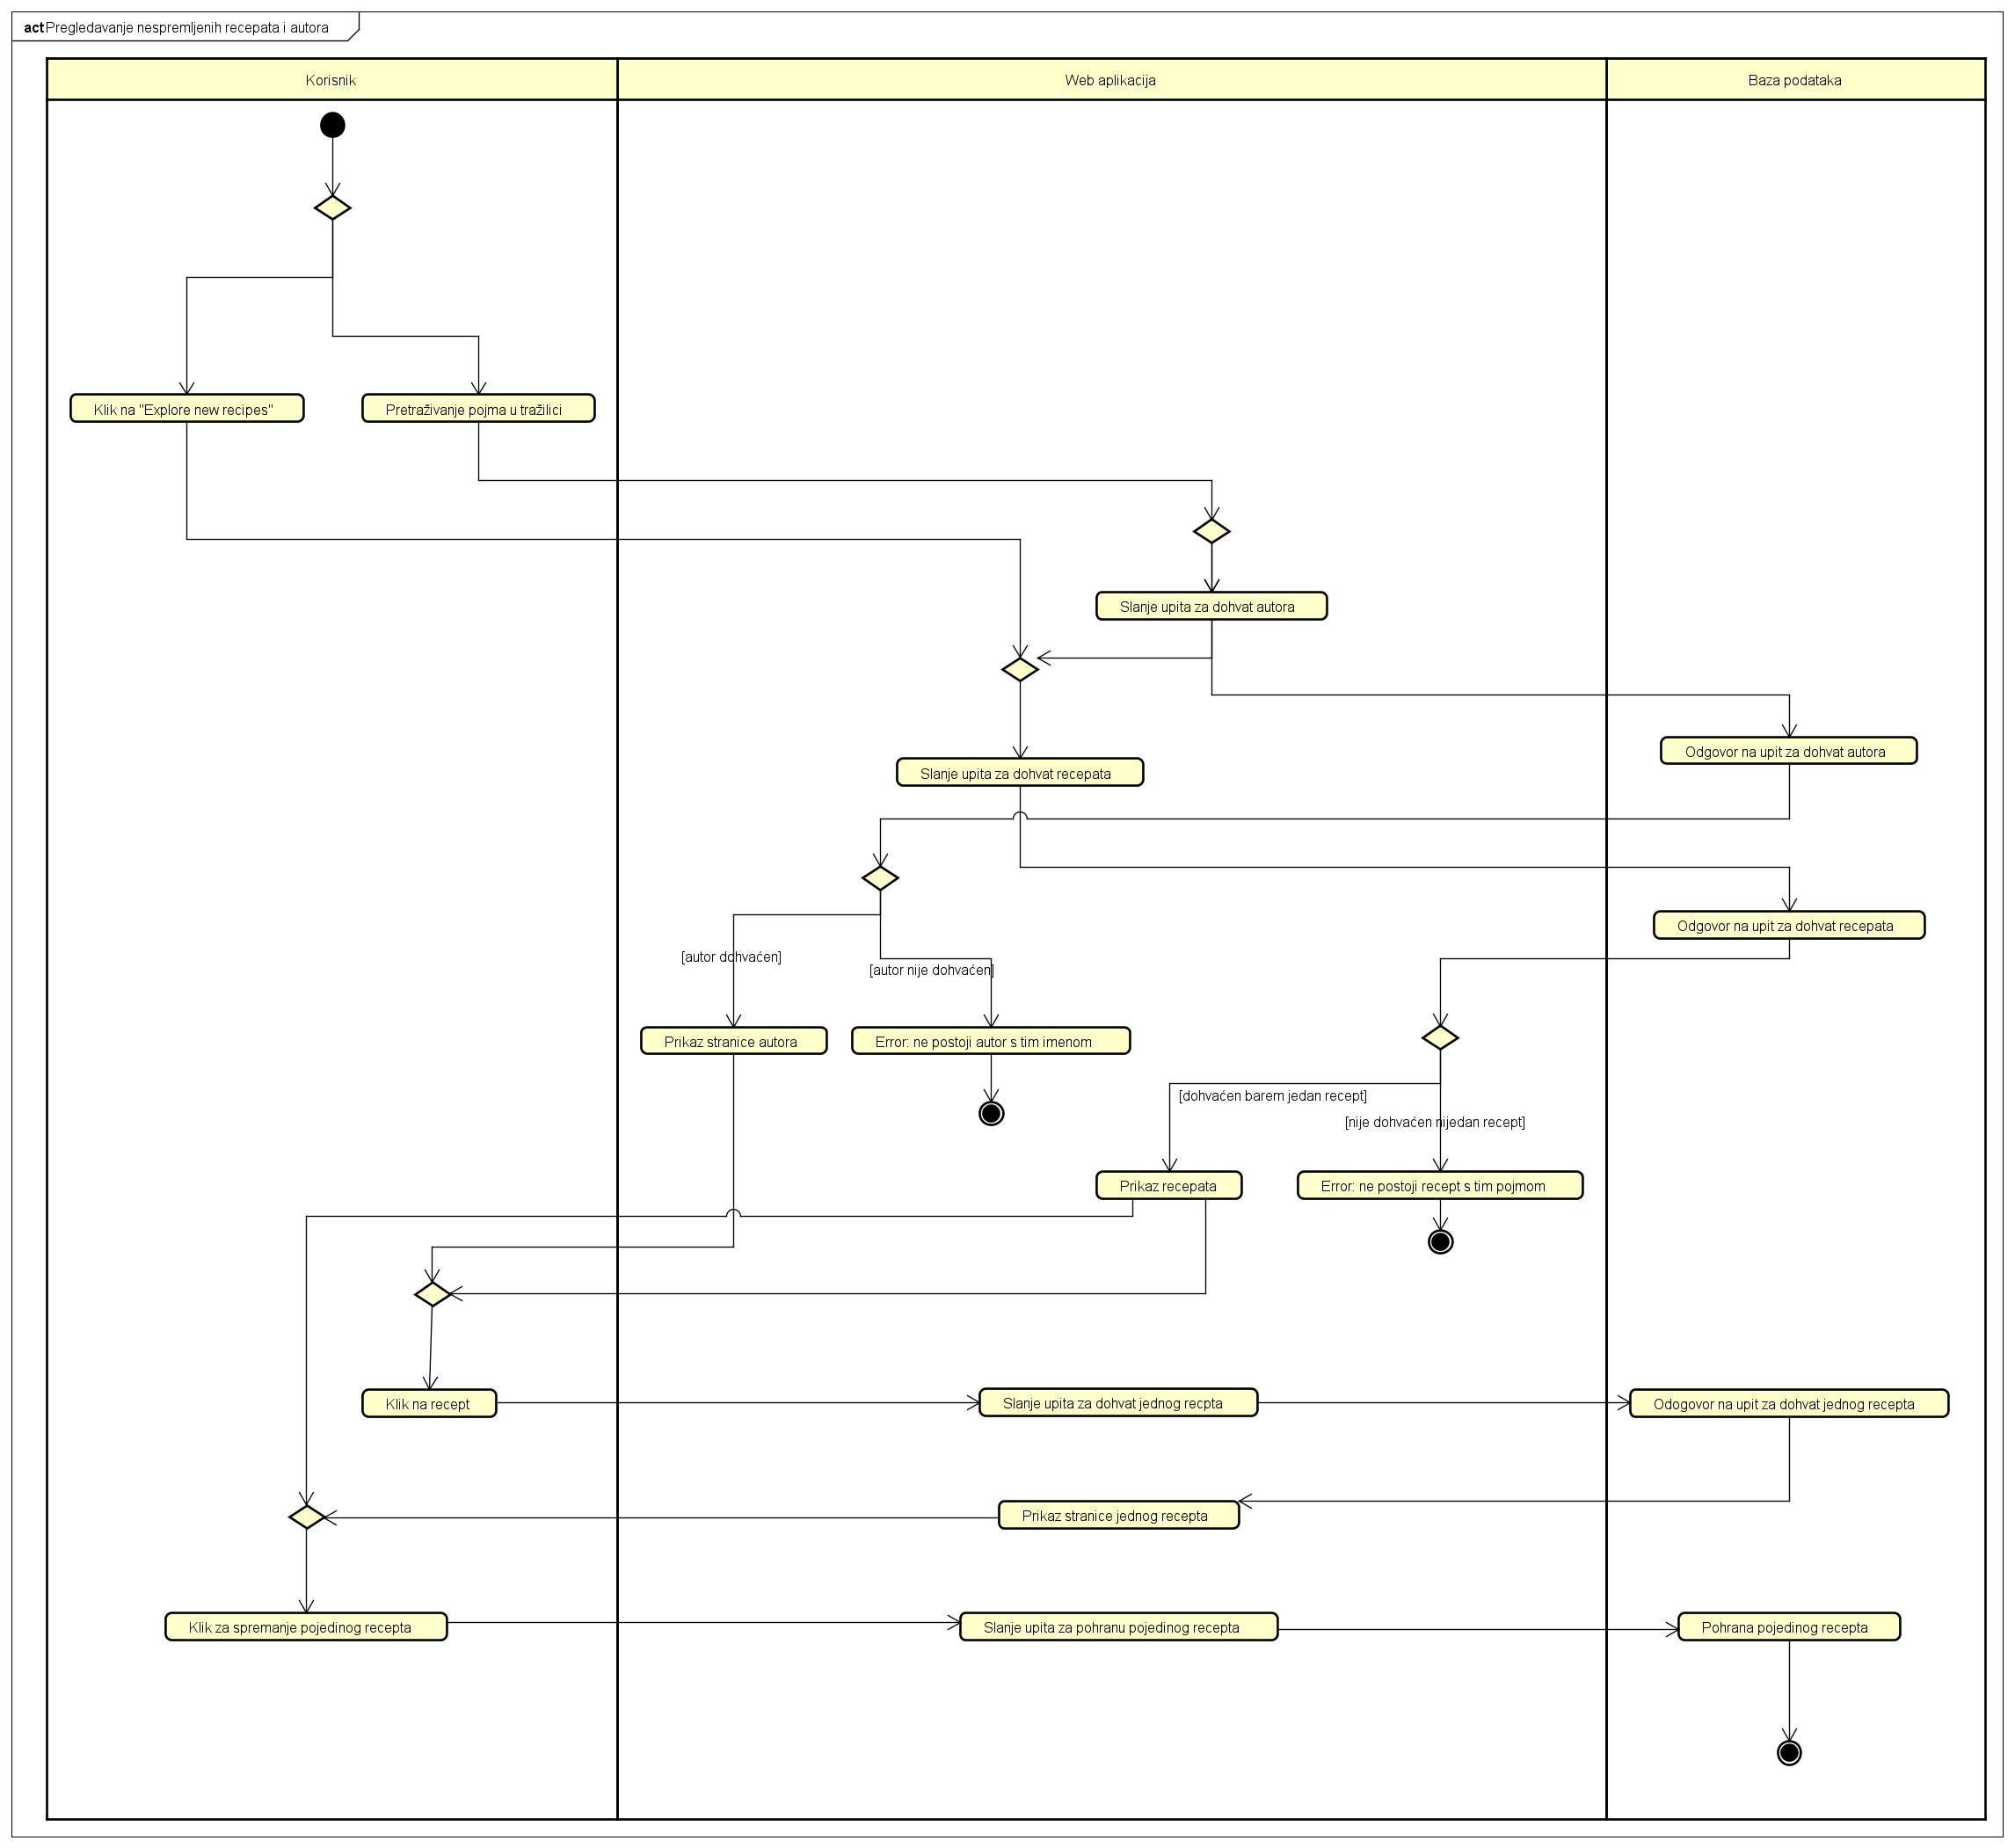
\includegraphics[width=1\textwidth]{slike/dijagrami/Pregledavanje nespremljenih recepata i autora_dijagram_aktivnosti.png}
				\caption{Dijagram aktivnosti za pregledavanje nespremljenih recepata i autora}
				\label{fig:enter-label}
			\end{figure}
			
			\eject

		\section{Dijagram komponenti}
		
		\noindent Dijagram komponenti
			
			\begin{figure}[H]
				\centering
				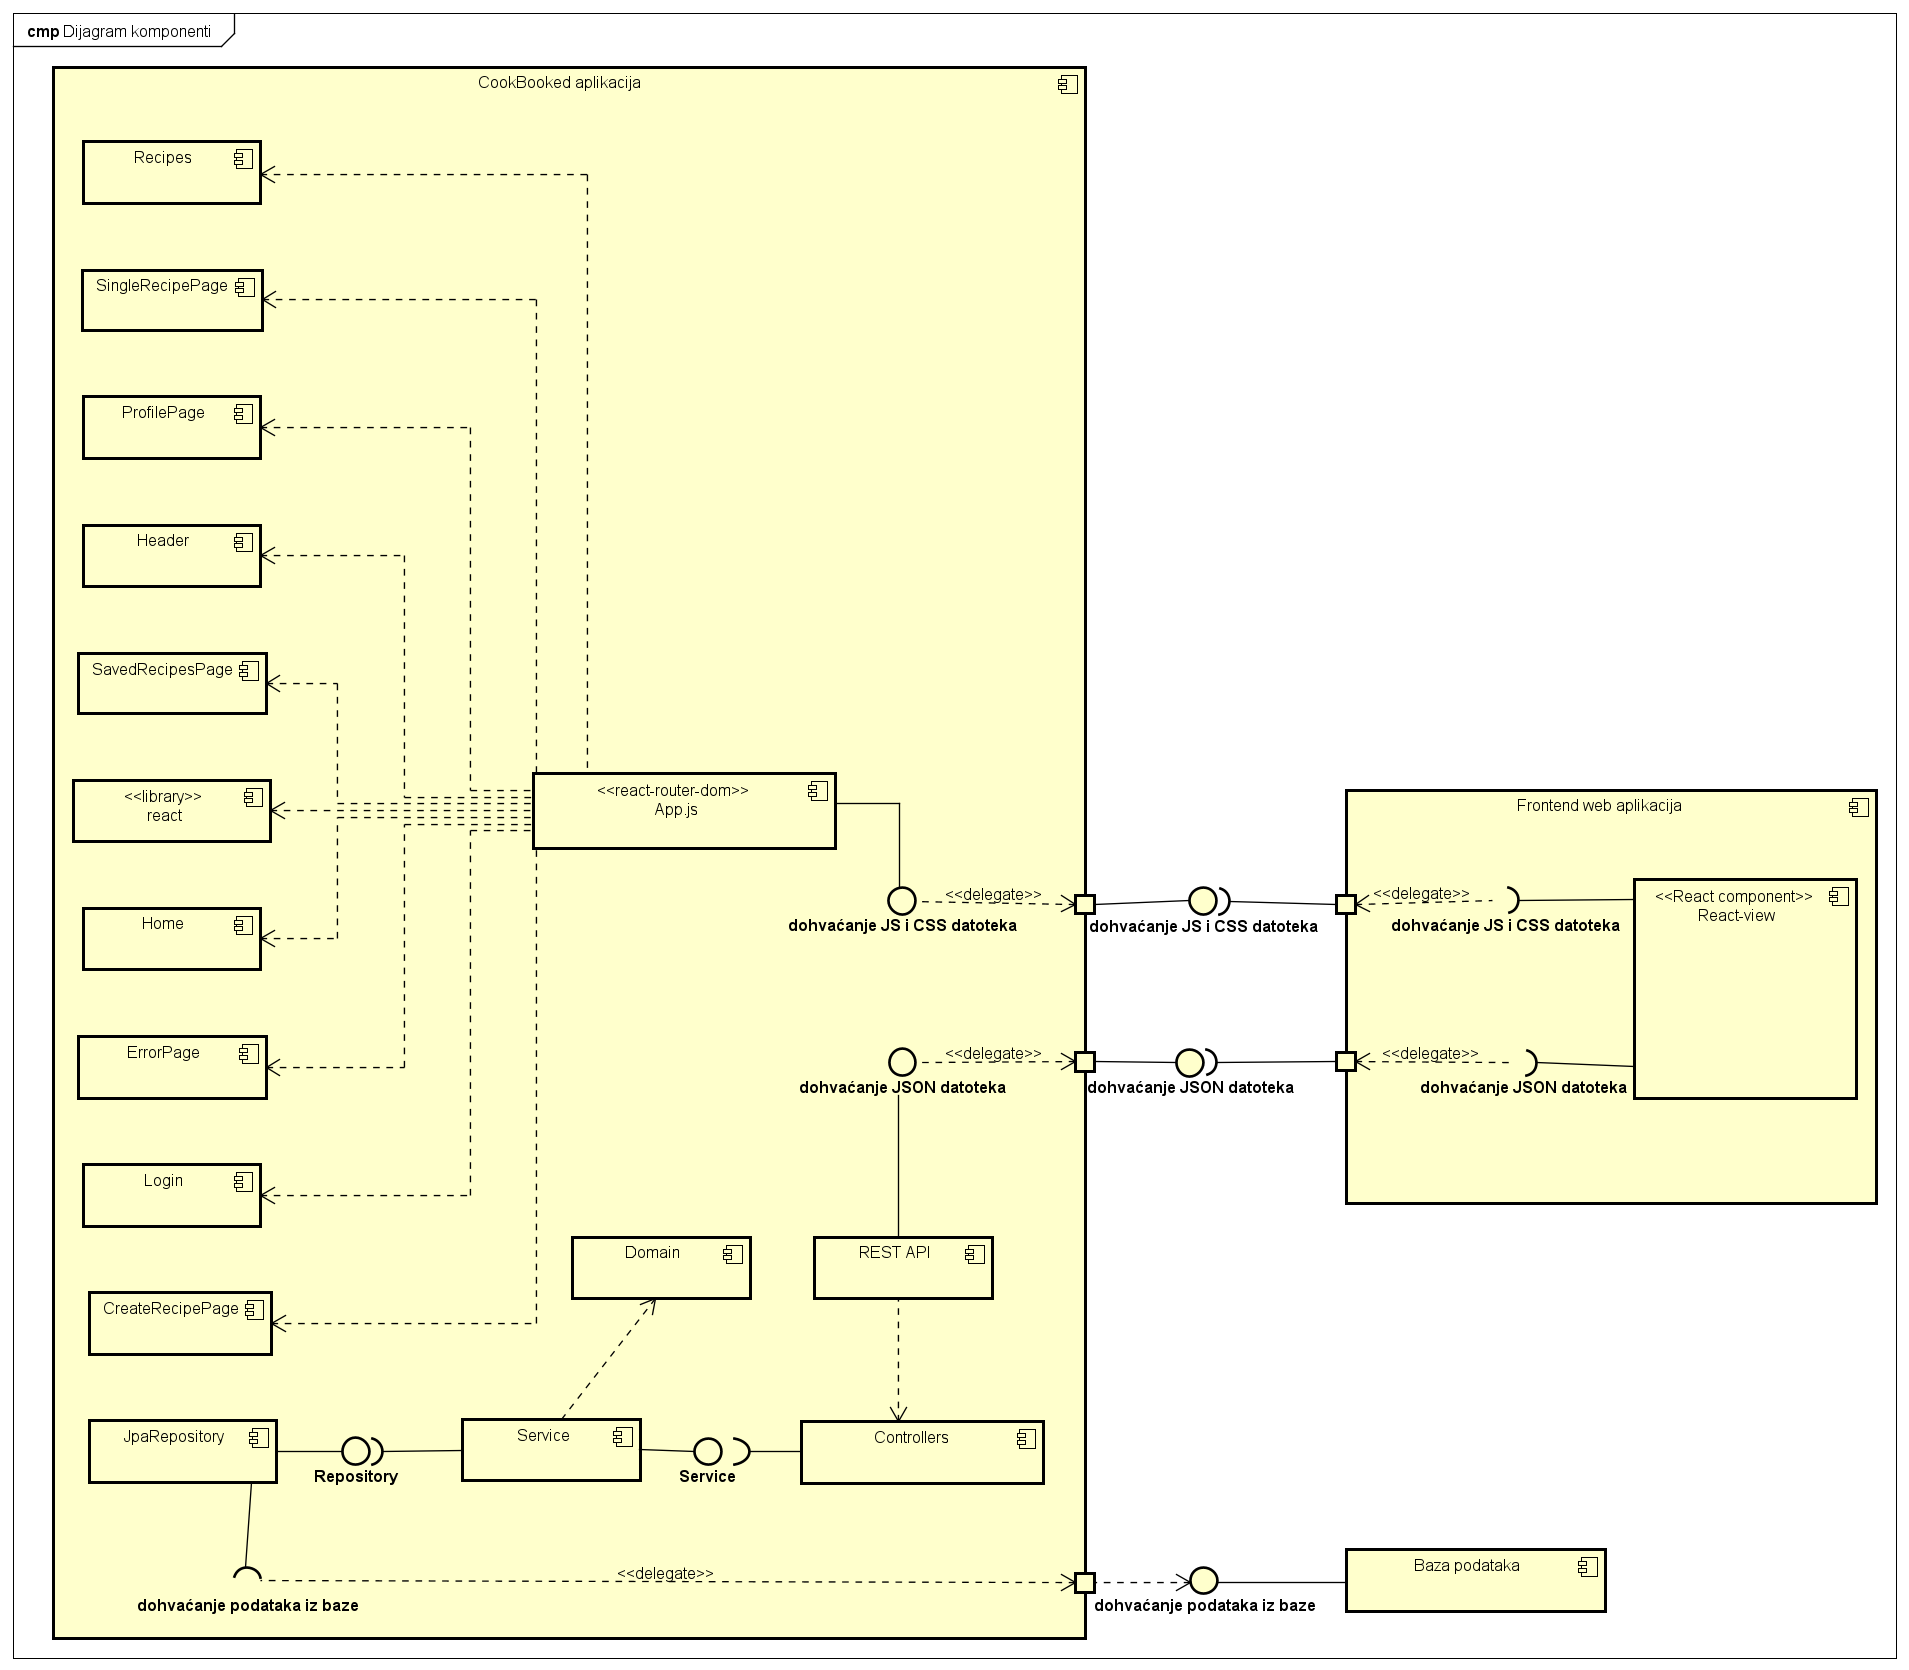
\includegraphics[width=1\textwidth]{slike/dijagrami/Dijagram komponenti.png}
				\caption{Dijagram komponenti}
				\label{fig:enter-label}
			\end{figure}
	\chapter{Implementacija i korisničko sučelje}
		
		
		\section{Korištene tehnologije i alati}
		
			% \textbf{\textit{dio 2. revizije}}
			
			%  \textit{Detaljno navesti sve tehnologije i alate koji su primijenjeni pri izradi dokumentacije i aplikacije. Ukratko ih opisati, te navesti njihovo značenje i mjesto primjene. Za svaki navedeni alat i tehnologiju je potrebno \textbf{navesti internet poveznicu} gdje se mogu preuzeti ili više saznati o njima}.
			\noindent Projekt je izveden primjenom različitih tehnologija i alata u svrhu implementacije kao i za dokumentaciju. U nastavku slijedi lista alata i tehnologija koje smo koristili uz kratke opise njihove uporabe.
			\newline\newline
			\noindent\textbf{VisualStudioCode}\footnote[1]{https://code.visualstudio.com/} je besplatni visoko prilagodljiv tekstualni editor namijenjen širokom spektru programskih jezika i platformi. U sklopu ovoga projekta koristio se za pri pomoći u izradi dokumentacije. \textbf{LaTeX}\footnote[2]{https://www.latex-project.org/} je visokokvalitetan sustav za pisanje teksta koji se koristi za izradu tehničkih i znanstvenih dokumentacija zato što pruža konzistentan izgled dokumenta. Dokumentacija ovog projekta pisana je u LaTeX-u uporabom različitih okruženja kao što su \textbf{TeXStudio}\footnote[3]{https://www.texstudio.org/} (integrirano okruženje koje pruža sučelje za jednostavno pisanje, uređivanje i kompiliranje LaTeX koda), \textbf{Overleaf}\footnote[4]{https://www.overleaf.com/} (online suradnički editor koji omogućuje zajednički rad više korisnika na istom dokumentu u stvarnom vremenu) i \textbf{LaTeX Workshop}\footnote[5]{https://marketplace.visualstudio.com/items?itemName=James-Yu.latex-workshop} (extension unutar VSC-a koji pruža potpore za pisanje, uređivanje i kompiliranje LaTeX koda). Za izradu dijagrama korišten je \textbf{Astah}\footnote[6]{https://astah.net/} alat za modeliranje UML dijagrama. To je alat koji omogućuje vizualno prikazivanje struktura, interakcija i dinamike sustava što pomaže pri razumijevanju i planiranju arhitekture aplikacija. Također, dio dijagrama iscrtan je pomoću web-aplikacije za crtanje dijagrama \textbf{draw.io}\footnote[7]{https://app.diagrams.net/} koja pruža mogućnosti kao i Astah uz intuitivno korisničko sučelje koje olakšava vizualizaciju i komunikaciju ideja.
			\newline\newline
			\noindent\textbf{PostgreSQL}\footnote[8]{https://www.postgresql.org/} je snažan, open-source sustav za upravljanje bazama podataka koji podržava relacijski model podataka. Ova baza pruža napredne značajke poput transakcija, podrške za vanjske ključeve, indeksiranja i proširivosti. U ovome projektu PostgreSQL je korišten unutar integriranog razvojnog okruženja \textbf{DataGrip}\footnote[9]{https://www.jetbrains.com/datagrip/} koji nudi napredne alate uz brzu navigaciju, pisanje i testiranje SQL upita, upravljanje shemama i izvođenje drugih zadataka nad bazom podataka. Od ponuđenih administratorskih alata koristio se \textbf{pgAdmin4}\footnote[10]{https://www.pgadmin.org/download/} koji omogućuje korisnicima pregled i manipulaciju bazom, shemama, tablicama i drugim objektima. Za izradu relacijskog modela baze podataka korišten je \textbf{ERDPlus}\footnote[11]{https://erdplus.com/} besplatni online programski alat koji omogućuje izradu i uređivanje dijagrama baze podataka te njihov izvoz u .png formatu.
			\newline\newline
			\noindent\textbf{IntelliJ IDEA}\footnote[12]{https://www.jetbrains.com/idea/} je integrirano razvojno okruženje namijenjeno potpori razvoju softvera u različitim programskim jezicima s naglaskom na Javi. Ono pruža bogat skup alata za pisanje koda, rafaktoriranje i debagiranje, a podržava širok spektar tehnologija. Backend razvoj ovog projekta izveden je unutar IntelliJ IDEA razvojne okoline upotrebom \textbf{Java}\footnote[13]{https://www.java.com/en/} objektno orijentiranog programskog jezika u radnom okviru \textbf{Spring Boot}\footnote[14]{https://spring.io/projects/spring-boot/} (otvoreni okvir za razvoj Java aplikacija koji pruža konvencije nad konfiguracijama, ugrađene funkcionalnosti poput ugrađenog servera i podršku za mikroservere). Za ispitivanje funkcionalnosti backenda koristila se \textbf{Postman}\footnote[15]{https://www.postman.com/} platforma za suradnju u razvoju API-ja. Ovaj alat pruža korisničko sučelje za stvaranje, testiranje i upravljanje HTTP API zahtjevima i odgovorima.
			\newline\newline
			\noindent\textbf{WebStorm}\footnote[16]{https://www.jetbrains.com/webstorm/?var=1} je integrirano razvojno okruženje dizajnirano za web razvoj koje pruža napredne značajke kao što su automatsko dovršavanje koda, analiza u stvarnom vremenu, duboko integriranje s alatima za sustave za upravljanje verzijama i drugim alatima za web razvoj. Frontend se razvijao unutar WebStorm-a upotrebom označnog jezika \textbf{HTML}\footnote[17]{https://www.w3schools.com/html/} (za prikaz sadržaja na web-u), stilskog jezika \textbf{CSS}\footnote[18]{https://www.w3schools.com/css/} (koji se koristi za opis izgleda i drugih stilskih karakteristika na web-u) i skriptnog programskog jezika \textbf{JavaScript}\footnote[19]{https://www.javascript.com/} (koji se u web pregledniku izvršava na strani korisnika) te njegove biblioteke otvorenog koda \textbf{ReactJS}\footnote[20]{https://react.dev/} (koja se koristi za komponentni pristup razvoju i učinkovito ažuriranje sučelja bez potrebe za punim ponovnim iscrtavanjem).
			\newline\newline
			\noindent\textbf{GitHub}\footnote[21]{https://github.com/} je online platforma korištena za upravljanje projektom i pohranu programskog koda i dokumentacije, a oslanja se na Git verzioniranje koda. Ona omogućuje suradnju među članovima grupe, olakšava praćenje zadataka, zaduženja i promjena na projektu te razvoj na posebnim granama i njihovo spajanje. \textbf{GitHub Desktop}\footnote[22]{https://desktop.github.com/} je besplatna aplikacija koja olakšava upotrebu Git-a s intuitivnim sučeljem koje olakšava dodavanje vlastitih promjena u repozitorij projekta. Korištena je kao alat za dodavanje i dohvaćanje podataka projekta. Za komunikaciju o detaljima projekta i raspodjelu posla i zadataka te međusobnu pomoć u izvođenju istih, tim je koristio \textbf{Discord}\footnote[23]{https://discord.com/} server. Discord je platforma za komunikaciju putem glasovnih, video i tekstualnih razgovora, a omogućuje izradu različitih kanala za organizirano komuniciranje.
			
			\eject 
		
	
		\section{Ispitivanje programskog rješenja}
			
			\textbf{\textit{dio 2. revizije}}\\
			
			 \textit{U ovom poglavlju je potrebno opisati provedbu ispitivanja implementiranih funkcionalnosti na razini komponenti i na razini cijelog sustava s prikazom odabranih ispitnih slučajeva. Studenti trebaju ispitati temeljnu funkcionalnost i rubne uvjete.}
	
			
			\subsection{Ispitivanje komponenti}
			\textit{Potrebno je provesti ispitivanje jedinica (engl. unit testing) nad razredima koji implementiraju temeljne funkcionalnosti. Razraditi \textbf{minimalno 6 ispitnih slučajeva} u kojima će se ispitati redovni slučajevi, rubni uvjeti te izazivanje pogreške (engl. exception throwing). Poželjno je stvoriti i ispitni slučaj koji koristi funkcionalnosti koje nisu implementirane. Potrebno je priložiti izvorni kôd svih ispitnih slučajeva te prikaz rezultata izvođenja ispita u razvojnom okruženju (prolaz/pad ispita). }
			
			
			
			\subsection{Ispitivanje sustava}
			
			 \textit{Potrebno je provesti i opisati ispitivanje sustava koristeći radni okvir Selenium\footnote{\url{https://www.seleniumhq.org/}}. Razraditi \textbf{minimalno 4 ispitna slučaja} u kojima će se ispitati redovni slučajevi, rubni uvjeti te poziv funkcionalnosti koja nije implementirana/izaziva pogrešku kako bi se vidjelo na koji način sustav reagira kada nešto nije u potpunosti ostvareno. Ispitni slučaj se treba sastojati od ulaza (npr. korisničko ime i lozinka), očekivanog izlaza ili rezultata, koraka ispitivanja i dobivenog izlaza ili rezultata.\\ }
			 
			 \textit{Izradu ispitnih slučajeva pomoću radnog okvira Selenium moguće je provesti pomoću jednog od sljedeća dva alata:}
			 \begin{itemize}
			 	\item \textit{dodatak za preglednik \textbf{Selenium IDE} - snimanje korisnikovih akcija radi automatskog ponavljanja ispita	}
			 	\item \textit{\textbf{Selenium WebDriver} - podrška za pisanje ispita u jezicima Java, C\#, PHP koristeći posebno programsko sučelje.}
			 \end{itemize}
		 	\textit{Detalji o korištenju alata Selenium bit će prikazani na posebnom predavanju tijekom semestra.}
			
			\eject 
		
		
		\section{Dijagram razmještaja}
			
		\noindent Dijagram razmještaja prikazuje fizičku arhitekturu i konfiguraciju razmještaja našeg programskog sustava. Dijagrami razmještaja koji ne sadrže imena instanci nazivaju se specifikacijski dijagrami razmještaja. Korisnici koriste web preglednik kako bi mogli pristupiti web aplikaciji. Na poslužiteljskom računalu nalazi se web poslužitelj, a komunikacija između korisnika i poslužitelja se održava preko HTTP protokola. Baza podataka nalazi se na serveru, a o njoj, naravno, ovisi backend aplikacija s poslužiteljskog računala.
			
			\begin{figure}[H]
				\centering
				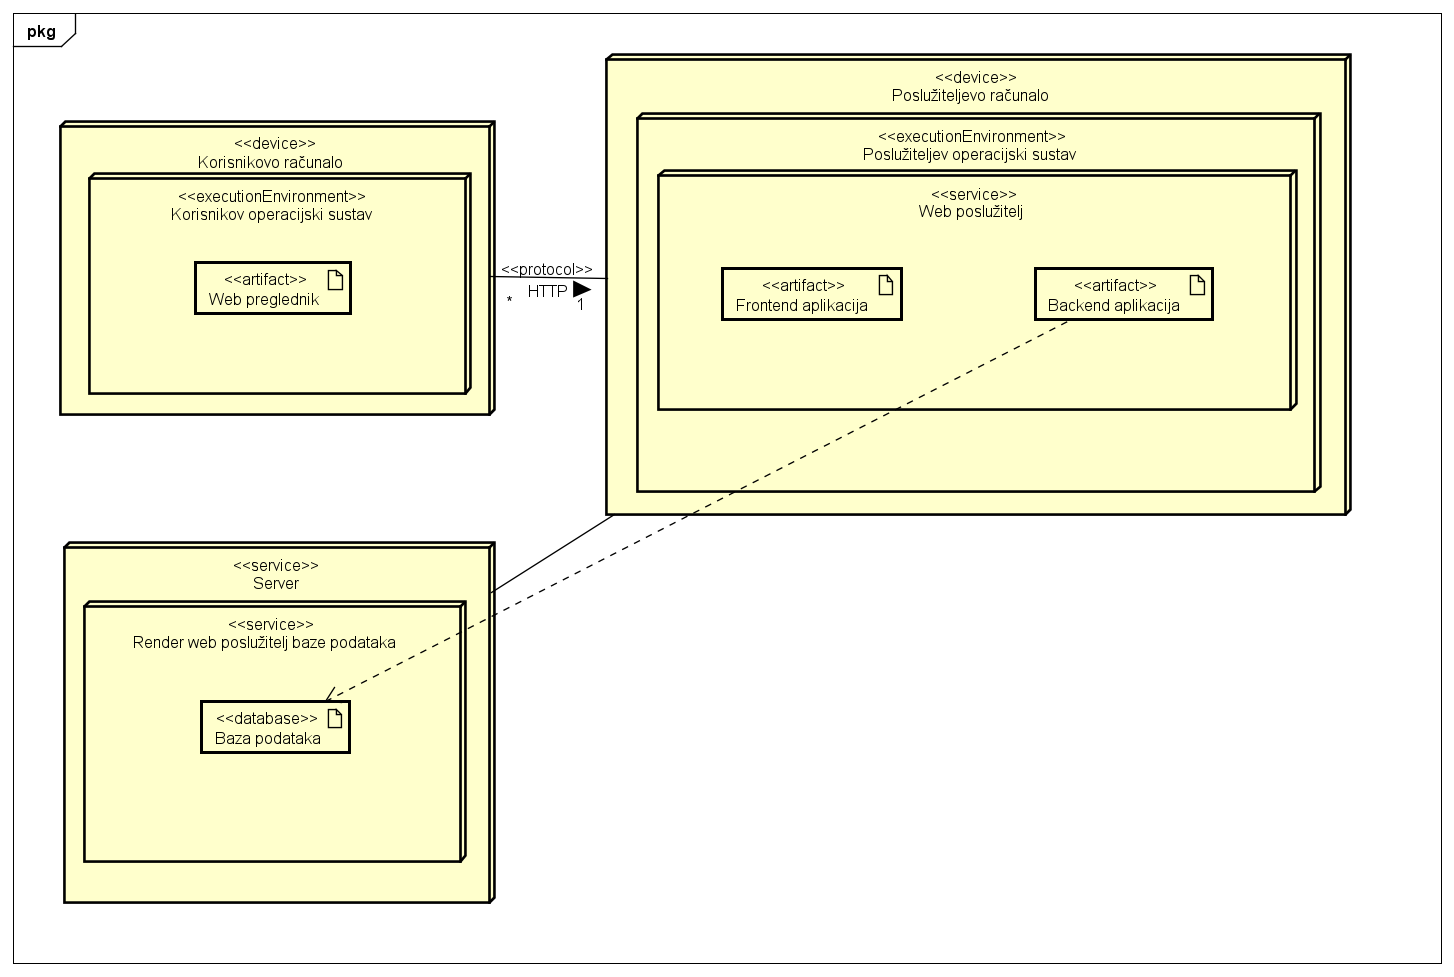
\includegraphics[width=1\textwidth]{slike/dijagrami/Dijagram razmjestaja.png}
				\caption{Dijagram razmještaja}
				\label{fig:enter-label}
			\end{figure}	

			\eject 
		
		\section{Upute za puštanje u pogon}
		
			% \textbf{\textit{dio 2. revizije}}\\
		
			%  \textit{U ovom poglavlju potrebno je dati upute za puštanje u pogon (engl. deployment) ostvarene aplikacije. Na primjer, za web aplikacije, opisati postupak kojim se od izvornog kôda dolazi do potpuno postavljene baze podataka i poslužitelja koji odgovara na upite korisnika. Za mobilnu aplikaciju, postupak kojim se aplikacija izgradi, te postavi na neku od trgovina. Za stolnu (engl. desktop) aplikaciju, postupak kojim se aplikacija instalira na računalo. Ukoliko mobilne i stolne aplikacije komuniciraju s poslužiteljem i/ili bazom podataka, opisati i postupak njihovog postavljanja. Pri izradi uputa preporučuje se \textbf{naglasiti korake instalacije uporabom natuknica} te koristiti što je više moguće \textbf{slike ekrana} (engl. screenshots) kako bi upute bile jasne i jednostavne za slijediti.}
			
			
			%  \textit{Dovršenu aplikaciju potrebno je pokrenuti na javno dostupnom poslužitelju. Studentima se preporuča korištenje neke od sljedećih besplatnih usluga: \href{https://aws.amazon.com/}{Amazon AWS}, \href{https://azure.microsoft.com/en-us/}{Microsoft Azure} ili \href{https://www.heroku.com/}{Heroku}. Mobilne aplikacije trebaju biti objavljene na F-Droid, Google Play ili Amazon App trgovini.}
			
			
			\eject 
	\chapter{Zaključak i budući rad}
		
		\textbf{\textit{dio 2. revizije}}\\
		
		 \textit{U ovom poglavlju potrebno je napisati osvrt na vrijeme izrade projektnog zadatka, koji su tehnički izazovi prepoznati, jesu li riješeni ili kako bi mogli biti riješeni, koja su znanja stečena pri izradi projekta, koja bi znanja bila posebno potrebna za brže i kvalitetnije ostvarenje projekta i koje bi bile perspektive za nastavak rada u projektnoj grupi.}
		 \noindent Izuzetno je mnogo vremena bilo potrošeno kako bi nadoknadili manjak jednog člana. Sve tehnologije koje smo koristili su nam bile nepoznate te smo zato čvsto odredili uloge kako bi smanjili obujam učenja pojedinog člana.
		 \noindent Backend je morao savladati Spring Boot i Maven sa svim svojim značajkama. Frontend je morao ovladati React-om za uređivanje komponenti stranice i npm-om za instalaciju paketa. Ljudi zaduženi za dokumentaciju su morali ovladati LaTex-om.
		 \noindent No kako to obično biva u malim timovima na kraju je svatko radio sve. Kada bi isti tim ljudi duže programirao zajedno te se dogovorio oko normi oblikovanja mogli bi biti brži i efektivniji, no to je bilo izuzetno teško sa našim popunjenim rasporedima.
		 \noindent Perspektiva koju smo svi usvojili je značajnost rada svakog od nas. Koliko god se pomoć činila mala na kraju bi njena značajnost imala veliku težinu.
		 \noindent \textbf{Ukratko, najbitnija je kontinuiranost u radu jer projekt iako kratak nije gotov u jednom danu.}
		 
		 \textit{Potrebno je točno popisati funkcionalnosti koje nisu implementirane u ostvarenoj aplikaciji.}
		 \noindent Unatoč volji, perspektivi te požrtvovnosti svih članova tima sljedeće značajke nismo uspijeli implementirati:
		\begin{itemize}
			\item video-chat između korisnika
			\item admin page (sa svojim značajkama)
			\item praćenje korisnika
			\item mijenjanje recepata
		\end{itemize}
		
		\eject 
	\chapter*{Popis literature}
		\addcontentsline{toc}{chapter}{Popis literature}
	 	
 		\textbf{\textit{Kontinuirano osvježavanje}}
	
		\textit{Popisati sve reference i literaturu koja je pomogla pri ostvarivanju projekta.}
		
		
		\begin{enumerate}
			
			
			\item  Programsko inženjerstvo, FER ZEMRIS, \url{http://www.fer.hr/predmet/proinz}
			
			\item  I. Sommerville, "Software engineering", 8th ed, Addison Wesley, 2007.
			
			\item  T.C.Lethbridge, R.Langaniere, "Object-Oriented Software Engineering", 2nd ed. McGraw-Hill, 2005.
			
			\item  I. Marsic, Software engineering book``, Department of Electrical and Computer Engineering, Rutgers University, \url{http://www.ece.rutgers.edu/~marsic/books/SE}
			
			\item  The Unified Modeling Language, \url{https://www.uml-diagrams.org/}
			
			\item  Astah Community, \url{http://astah.net/editions/uml-new}
		\end{enumerate}
		
		 
	
	
	\begingroup
	\renewcommand*\listfigurename{Indeks slika i dijagrama}
	%\renewcommand*\listtablename{Indeks tablica}
	%\let\clearpage\relax
	\listoffigures
	%\vspace{10mm}
	%\listoftables
	\endgroup
	\addcontentsline{toc}{chapter}{Indeks slika i dijagrama}


	
	\eject 
		
	\chapter*{Dodatak: Prikaz aktivnosti grupe}
		\addcontentsline{toc}{chapter}{Dodatak: Prikaz aktivnosti grupe}
		
		\section*{Dnevnik sastajanja}
		
		\textbf{\textit{Kontinuirano osvježavanje}}\\
		
		 \textit{U ovom dijelu potrebno je redovito osvježavati dnevnik sastajanja prema predlošku.}
		
		\begin{packed_enum}
			\item  sastanak
			
			\item[] \begin{packed_item}
				\item Datum: 19. listopada 2023.
				\item Prisustvovali: Dominik Dejanović, Ante Čavar, Borna Dramalija, Adam Vuković, Nikola Trebus, Ljubica Nikolić
				\item Teme sastanka:
				\begin{packed_item}
					\item  upoznavanje tima
					\item  raspodjela zadataka
					\item rasprava o korištenim tehnologijama
				\end{packed_item}
			\end{packed_item}
			
			\item  sastanak
			\item[] \begin{packed_item}
				\item Datum: 27. listopada 2023.
				\item Prisustvovali: Dominik Dejanović, Ante Čavar, Adam Vuković, Nikola Trebus, Volarević Volarević, Ljubica Nikolić
				\item Teme sastanka:
				\begin{packed_item}
					\item  dogovor oko dizajna baze podataka
					\item  dogovor oko rada na dokumentaiciji
					\item rasprava o budućim ciljevima
				\end{packed_item}
			\end{packed_item}
			
			%
			
		\end{packed_enum}
		
		\eject
		\section*{Tablica aktivnosti}
		
			%\textbf{\textit{Dokumentacija}}\\
			Aktivnost izražena u satima.

			\begin{longtblr}[
					label=none,
				]{
					vlines,hlines,
					width = \textwidth,
					colspec={X[7, l]X[1, c]X[1, c]X[1, c]X[1, c]X[1, c]X[1, c]X[1, c]}, 
					vline{1} = {1}{text=\clap{}},
					hline{1} = {1}{text=\clap{}},
					rowhead = 1,
				} 
			
				\SetCell[c=1]{c}{} & \SetCell[c=1]{c}{\rotatebox{90}{\textbf{Dominik Dejanović}}} & \SetCell[c=1]{c}{\rotatebox{90}{\textbf{Adam Vuković}}} &	\SetCell[c=1]{c}{\rotatebox{90}{\textbf{Ime Prezime }}} & \SetCell[c=1]{c}{\rotatebox{90}{\textbf{Ime Prezime }}} &	\SetCell[c=1]{c}{\rotatebox{90}{\textbf{Ime Prezime }}} & \SetCell[c=1]{c}{\rotatebox{90}{\textbf{Ime Prezime }}} &	\SetCell[c=1]{c}{\rotatebox{90}{\textbf{Ime Prezime }}} \\  
				Upravljanje projektom 		& 2  &  &  &  &  &  & \\ 
				Opis projektnog zadatka 	&  &  3  &  &  &  & \\ 
				
				Funkcionalni zahtjevi       &  &  &  &  &  &  &  \\ 
				Opis pojedinih obrazaca 	& 3  &  &  &  &  &  &  \\ 
				Dijagram obrazaca 			& 1  &  &  &  &  &  &  \\ 
				Sekvencijski dijagrami 		& 1  &  &  &  &  &  &  \\ 
				Opis ostalih zahtjeva 		&  &  &  &  &  &  &  \\ 

				Arhitektura i dizajn sustava	 &  &  &  &  &  &  &  \\ 
				Baza podataka				&  &  &  &  &  &  &   \\ 
				Dijagram razreda 			&  &  &  &  &  &  &   \\ 
				Dijagram stanja				&  &  &  &  &  &  &  \\ 
				Dijagram aktivnosti 		&  &  &  &  &  &  &  \\ 
				Dijagram komponenti			&  &  &  &  &  &  &  \\ 
				Korištene tehnologije i alati 		&  &  &  &  &  &  &  \\ 
				Ispitivanje programskog rješenja 	&  &  &  &  &  &  &  \\ 
				Dijagram razmještaja			&  &  &  &  &  &  &  \\ 
				Upute za puštanje u pogon 		&  &  &  &  &  &  &  \\  
				Dnevnik sastajanja 			& 1  &  &  &  &  &  &  \\ 
				Zaključak i budući rad 		&  &  &  &  &  &  &  \\  
				Popis literature 			&  &  &  &  &  &  &  \\  
				Web stranica & 3  &  &  &  &  &  & \\
				&  &  &  &  &  &  &  \\ \hline 
				\textit{Dodatne stavke kako ste podijelili izradu aplikacije} 			&  &  &  &  &  &  &  \\ 
				\textit{npr. izrada početne stranice} 				&  &  &  &  &  &  &  \\  
				\textit{izrada baze podataka} 		 			&  &  &  &  &  &  & \\  
				\textit{spajanje s bazom podataka} 							&  &  &  &  &  &  &  \\ 
				\textit{back end} 							&  &  &  &  &  &  &  \\  
				 							&  &  &  &  &  &  &\\ 
			\end{longtblr}
					
					
		\eject
		\section*{Dijagrami pregleda promjena}
		
		\textbf{\textit{dio 2. revizije}}\\
		
		\textit{Prenijeti dijagram pregleda promjena nad datotekama projekta. Potrebno je na kraju projekta generirane grafove s gitlaba prenijeti u ovo poglavlje dokumentacije. Dijagrami za vlastiti projekt se mogu preuzeti s gitlab.com stranice, u izborniku Repository, pritiskom na stavku Contributors.}
		
	


\end{document} %naredbe i tekst nakon ove naredbe ne ulaze u izgrađen dokument 


